% --------------------------------------------	
% This is an example 					
% Adding a customization Layer			
% Autogenerated LaTeX file for books 			
% --------------------------------------------	
\documentclass[spanish,french,english,a4paper,10pt,final]{report}
\label{book}\usepackage{ifthen}
% --------------------------------------------
% Check for PDFLaTeX/LaTeX 
% --------------------------------------------
\newif\ifpdf
\ifx\pdfoutput\undefined
\pdffalse % we are not running PDFLaTeX
\else
\pdfoutput=1 % we are running PDFLaTeX
\pdftrue
\fi
% --------------------------------------------
% Load graphicx package with pdf if needed 
% --------------------------------------------
\ifpdf
\usepackage[pdftex]{graphicx}
\pdfcompresslevel=9
\else
\usepackage{graphicx}
\fi
\usepackage{anysize}
\marginsize{3cm}{2cm}{1.25cm}{1.25cm}
\usepackage{fancyhdr}
\pagestyle{fancy}
\renewcommand{\headrulewidth}{0.4pt}
\renewcommand{\footrulewidth}{0.4pt}
% ---------------------- 
% Most Common Packages   
% ---------------------- 
\usepackage{makeidx} 
\usepackage{varioref}         
\usepackage{latexsym}         
\usepackage{enumerate}         
\usepackage{fancybox}      
\usepackage{float}       
\usepackage{ragged2e}       
\usepackage[french]{babel} 
\usepackage{fancyvrb}         
\makeatletter\@namedef{FV@fontfamily@default}{\def\FV@FontScanPrep{}\def\FV@FontFamily{}}\makeatother
\fvset{obeytabs=true,tabsize=3}
\usepackage{isolatin1}         
\usepackage{rotating}         
\usepackage{subfigure}         
\usepackage{tabularx}         
\usepackage{url}         
 \def\keywords{\vspace{-.3em}
 \if@twocolumn
 \small{\itshape 
Keywords }\/\bfseries---$\!$%
 \else
 \begin{center}\small\bfseries 
Keywords \end{center}\quotation\small
 \fi}
 \def\endkeywords{\vspace{0.6em}\par\if@twocolumn\else\endquotation\fi
 \normalsize\rmfamily}
% --------------------------------------------
% Math support                                
% --------------------------------------------
\usepackage{amsmath,amsthm, amsfonts, amssymb, amsxtra,amsopn}
%\newtheorem{thm}{Theorem}[section]
%\newtheorem{cor}[section]{Corollary}
%\newtheorem{lem}[section]{Lemma}
%\newtheorem{defn}[section]{Definition}
%\newtheorem{prop}[section]{Proposition}
%\newtheorem{ax}{Axiom}
%\newtheorem{theorem}[section]{Theorem}
%\newtheorem{corollary}{Corollary}
%\newtheorem{lemma}{Lemma}
%\newtheorem{proposition}{Proposition}
%\theoremstyle{definition}
%\newtheorem{definition}{Definition}
%\theoremstyle{remark}
%\newtheorem{rem}{Remark}
%\newtheorem*{notation}{Notation}
%\newcommand{\ntt}{\normalfont\ttfamily}
%\newcommand{\thmref}[1]{Theorem~\ref{#1}}
%\newcommand{\secref}[1]{\S\ref{#1}}
%\newcommand{\lemref}[1]{Lemma~\ref{#1}}
 \newcommand{\bysame}{\mbox{\rule{3em}{.4pt}}\,}
 \newcommand{\A}{\mathcal{A}}
 \newcommand{\B}{\mathcal{B}}
 \newcommand{\XcY}{{(X,Y)}}
 \newcommand{\SX}{{S_X}}
 \newcommand{\SY}{{S_Y}}
 \newcommand{\SXY}{{S_{X,Y}}}
 \newcommand{\SXgYy}{{S_{X|Y}(y)}}
 \newcommand{\Cw}[1]{{\hat C_#1(X|Y)}}
 \newcommand{\G}{{G(X|Y)}}
 \newcommand{\PY}{{P_{\mathcal{Y}}}}
 \newcommand{\X}{\mathcal{X}}
 \newcommand{\wt}{\widetilde}
 \newcommand{\wh}{\widehat}
 % --------------------------------------------
 \DeclareMathOperator{\per}{per}
 \DeclareMathOperator{\cov}{cov}
 \DeclareMathOperator{\non}{non}
 \DeclareMathOperator{\cf}{cf}
 \DeclareMathOperator{\add}{add}
 \DeclareMathOperator{\Cham}{Cham}
 \DeclareMathOperator{\IM}{Im}
 \DeclareMathOperator{\esssup}{ess\,sup}
 \DeclareMathOperator{\meas}{meas}
 \DeclareMathOperator{\seg}{seg}
% --------------------------------------------
% --------------------------------------------
% Load hyperref package with pdf if needed 
% --------------------------------------------
\ifpdf
\usepackage[pdftex,bookmarksnumbered,colorlinks,backref, bookmarks, breaklinks, linktocpage,]{hyperref}
\else
\usepackage[dvips,bookmarksnumbered,colorlinks,backref, bookmarks, breaklinks, linktocpage,]{hyperref}
\fi
% --------------------------------------------
\newenvironment{admminipage}{\begin{Sbox}\begin{minipage}}{\end{minipage}\end{Sbox}\fbox{\TheSbox}}
\newlength{\admlength}
\newenvironment{admonition}[2] {
 \hspace{0mm}\newline\newline
 \noindent
 \setlength{\fboxsep}{5pt}
 \setlength{\admlength}{\linewidth}
 \addtolength{\admlength}{-10\fboxsep}
 \addtolength{\admlength}{-10\fboxrule}
 \admminipage{\admlength}
 {\bf \sc\large{#2}} \newline
 \\[1mm]
 \sffamily
 \includegraphics[width=1cm]{#1}
 \addtolength{\admlength}{-1cm}
 \addtolength{\admlength}{-20pt}
 \begin{minipage}[lt]{\admlength}
 \parskip=0.5\baselineskip \advance\parskip by 0pt plus 2pt
}{
 \vspace{5mm} 
 \end{minipage}
 \endadmminipage
 \vspace{.5em}
 \newline
}
% --------------------------------------------
% Commands to manage/style/create floats      
% figures, tables, algorithms, examples, eqn  
% --------------------------------------------
 \floatstyle{ruled}
 \restylefloat{figure}
 \floatstyle{ruled}
 \restylefloat{table}
 \floatstyle{ruled}
 \newfloat{program}{ht}{lop}[section]
 \floatstyle{ruled}
 \newfloat{example}{ht}{loe}[section]
 \floatname{example}{Example}
 \floatstyle{ruled}
 \newfloat{dbequation}{ht}{loe}[section]
 \floatname{dbequation}{Equation}
 \floatstyle{boxed}
 \newfloat{algorithm}{ht}{loa}[section]
 \floatname{algorithm}{Algorithm}
\ifpdf
\DeclareGraphicsExtensions{.pdf,.png,.jpg}
\else
\DeclareGraphicsExtensions{.eps}
\fi
% --------------------------------------------
% A way to honour <footnoteref>s
% Blame j-devenish (at) users.sourceforge.net
% In any other LaTeX context, this would probably go into a style file.
\makeatletter
\newcommand{\docbooktolatexusefootnoteref}[1]{\@ifundefined{@fn@label@#1}%
  {\hbox{\@textsuperscript{\normalfont ?}}%
    \@latex@warning{Footnote label `#1' was not defined}}%
  {\@nameuse{@fn@label@#1}}}
\newcommand{\docbooktolatexmakefootnoteref}[1]{%
  \protected@write\@auxout{}%
    {\global\string\@namedef{@fn@label@#1}{\@makefnmark}}%
  \@namedef{@fn@label@#1}{\hbox{\@textsuperscript{\normalfont ?}}}%
  }
\makeatother% --------------------------------------------
% Hacks for honouring row/entry/@align
% (\hspace not effective when in paragraph mode)
% Naming convention for these macros is:
% 'docbooktolatex' 'align' {alignment-type} {position-within-entry}
% where r = right, l = left, c = centre
\newcommand{\docbooktolatexalignrl}{\protect\ifvmode\raggedleft\else\hfill\fi}
\newcommand{\docbooktolatexalignrr}{\protect}
\newcommand{\docbooktolatexalignll}{\protect\ifvmode\raggedright\else\fi}
\newcommand{\docbooktolatexalignlr}{\protect\ifvmode\else\hspace*\fill\fi}
\newcommand{\docbooktolatexaligncl}{\protect\ifvmode\centering\else\hfill\fi}
\newcommand{\docbooktolatexaligncr}{\protect\ifvmode\else\hspace*\fill\fi}
% --------------------------------------------
% Little Trick For Scaping!!!!!!
\newcommand{\docbooktolatexbackslash}{\textbackslash{}}
% --------------------------------------------
% $latex.caption.swapskip enabled for $formal.title.placement support
\newlength{\docbooktolatextempskip}
\newcommand{\captionswapskip}{\setlength{\docbooktolatextempskip}{\abovecaptionskip}\setlength{\abovecaptionskip}{\belowcaptionskip}\setlength{\belowcaptionskip}{\docbooktolatextempskip}}
\title{\bfseries Th�ses et Th�sards}
\author{Norman Walsh \and Ramon Casellas \and James Devenish}
% --------------------------------------------
\makeindex
\makeglossary
% --------------------------------------------

\setcounter{tocdepth}{4}

\setcounter{secnumdepth}{4}
\begin{document}

\InputIfFileExists{title}{\typeout{WARNING: Using cover pagetitle}}{\pagestyle{empty}\maketitle\pagestyle{fancy}}

% keywords ------------------------------------------------------
\begin{keywords}
KeyWord1, KeyWord2, KeyWord3 \end{keywords}
Copyright \copyright{} 1998 Norman Walsh [title] 
Legal Notice [/title] 

This is a test document. You can do what you will with it.

This is a second legal notice.  But it's not noteworthy.
  Some more text. Some more text. Some more text. Some more text. 
  Some more text. Some more text. Some more text. Some more text. 
  Some more text. Some more text. Some more text. Some more text. 
  Some more text. Some more text. Some more text. Some more text. 
  Some more text. Some more text. Some more text. Some more text. 
  Some more text. Some more text. Some more text. Some more text. 
  Some more text. Some more text. Some more text. Some more text. 
  
% -------------------------------------------------------------
% Dedication	 
% -------------------------------------------------------------
\label{id2718911}\newpage

{\sc Dedication}

\paragraph*{}
This test book is dedicated to all the testers.  This is the first para
of the dedication.
\paragraph*{}
This is the second para of the dedication.
\paragraph*{}
This is the third para of the dedication.
% ------------------------------------------------------------
% Preface
% ------------------------------------------------------------
\label{id2718928}
\chapter*{Preface Title}

Preface content.

This is the second para of the preface.

This is the third para of the preface.

\tableofcontents
% ------------------------------------------------------------- 
% 
% PART Part One Title
% 
% ------------------------------------------------------------- 
\part{Part One Title}
\label{id2767353}\hypertarget{id2767353}{}%

% -------------------------------------------------------------
% Chapter XRef Tests 
% ------------------------------------------------------------- 	
\chapter{XRef Tests}
\label{chapter}\hypertarget{chapter}{}%

\subsubsection*{Xrefs}\label{id2767430}

\vspace{1cm}
\begin{tabular*}{\linewidth}{l}
\hyperlink{book}{{\em Th�ses et Th�sards}}  \\
\hyperlink{part}{Part {\ref*{part}}}  \\
\hyperlink{chapter}{Chapter {\ref*{chapter}}, {\em XRef Tests}}  \\
\hyperlink{appendix}{Appendix {\ref*{appendix}}}  \\
\hyperlink{table}{Table {\ref*{table}}}  \\
\hyperlink{figure}{Figure {\ref*{figure}}}  \\
\hyperlink{example}{Example {\ref*{example}}}  \\
\hyperlink{equation}{Equation {\ref*{equation}}}  \\
\hyperlink{reference}{Reference {\ref*{reference}}}  \\
\hyperlink{bib1}{``A Test Bibliography''}  \\
\hyperlink{gloss}{``Example Glossary''}  \\
\hyperlink{index}{``Index''}  \\
\end{tabular*}
\vspace{1cm}

this is a test of \href{http://www.enst.fr}{ENST}

\vspace{1cm}
\begin{tabular*}{\linewidth}{ll}
\hyperlink{book}{{\em Th�ses et Th�sards}} & \hyperlink{example}{Example {\ref*{example}}}  \\
\hyperlink{part}{Part {\ref*{part}}} & \hyperlink{equation}{Equation {\ref*{equation}}}  \\
\hyperlink{chapter}{Chapter {\ref*{chapter}}, {\em XRef Tests}} & \hyperlink{reference}{Reference {\ref*{reference}}}  \\
\hyperlink{appendix}{Appendix {\ref*{appendix}}} & \hyperlink{bib1}{``A Test Bibliography''}  \\
\hyperlink{table}{Table {\ref*{table}}} & \hyperlink{gloss}{``Example Glossary''}  \\
\hyperlink{figure}{Figure {\ref*{figure}}} & \hyperlink{index}{``Index''}  \\
\end{tabular*}
\vspace{1cm}

this is a test of \href{http://www.enst.fr}{ENST}

This is the first reference to {\em XML}.
This is the second reference to XML.
These are references without linkend
attributes: {\em XML}, XML.

\subsubsection*{Links}\label{id2719565}

More \href{http://www.jclark.com/dsssl/}{DSSSL information}
is available.

There is \hyperlink{part}{a second part} in this book.

This is the \hyperlink{chapter}{XRef Tests}
chapter.

% -------------------------------------------------------------
% Chapter Section Tests 
% ------------------------------------------------------------- 	
\chapter{Section Tests}
\label{stchap}\hypertarget{stchap}{}%

some text. some text. some text. some text. some text. some text. 
some text. some text. some text. some text. some text. some text. some text. 
some text. some text. some text. some text. some text. some text. some text. 
some text. some text. some text. some text. some text. some text. some text. 
some text. some text. some text. some text. some text. some text. some text. 
some text. some text. some text. some text. some text. some text. some text. 
\index{ap1}
\index{ap2}

\index{bp1!bp1bs1}
\index{bp2}

\index{cp1!cp1cs1!cp1cs1ct1}
\index{cp2}

\index{dp1!dp1ds1}
\index{dp1!dp1ds2}
\index{dp2}

some text. some text. some text. some text. some text. some text. 
some text. some text. some text. some text. some text. some text. some text. 
some text. some text. some text. some text. some text. some text. some text. 
some text. some text. some text. some text. some text. some text. some text. 
some text. some text. some text. some text. some text. some text. some text. 
some text. some text. some text. some text. some text. some text. some text. 

some text. some text. some text. some text. some text. some text. 
some text. some text. some text. some text. some text. some text. some text. 
some text. some text. some text. some text. some text. some text. some text. 
some text. some text. some text. some text. some text. some text. some text. 
some text. some text. some text. some text. some text. some text. some text. 
some text. some text. some text. some text. some text. some text. some text. 

some text. some text. some text. some text. some text. some text. 
some text. some text. some text. some text. some text. some text. some text. 
some text. some text. some text. some text. some text. some text. some text. 
some text. some text. some text. some text. some text. some text. some text. 
some text. some text. some text. some text. some text. some text. some text. 
some text. some text. some text. some text. some text. some text. some text. 

% ------------------------   
% Section 
\section{a sect1 title}
\label{secttest1}\hypertarget{secttest1}{}%

some text. some text. some text. some text. some text. some text. 
some text. some text. some text. some text. some text. some text. some text. 
some text. some text. some text. some text. some text. some text. some text. 
some text. some text. some text. some text. some text. some text. some text. 
some text. some text. some text. some text. some text. some text. some text. 
some text. some text. some text. some text. some text. some text. some text. 
\index{ep1!ep1es1!ep1es1et1}
\index{ep1!ep1es2}
\index{ep2}

\index{fp1!fp1fs1}
\index{fp1!fp1fs2!fp1fs2ft1}
\index{fp2}

\index{gp1!gp1gs1}
\index{gp1!gp1gs2}
\index{gp1!gp1gs2!gp1gs2gt1}
\index{gp1!gp1gs2!gp1gs2gt2}
\index{gp1!gp1gs3}
\index{gp2}

some text. some text. some text. some text. some text. some text. 
some text. some text. some text. some text. some text. some text. some text. 
some text. some text. some text. some text. some text. some text. some text. 
some text. some text. some text. some text. some text. some text. some text. 
some text. some text. some text. some text. some text. some text. some text. 
some text. some text. some text. some text. some text. some text. some text. 

some text. some text. some text. some text. some text. some text. 
some text. some text. some text. some text. some text. some text. some text. 
some text. some text. some text. some text. some text. some text. some text. 
some text. some text. some text. some text. some text. some text. some text. 
some text. some text. some text. some text. some text. some text. some text. 
some text. some text. some text. some text. some text. some text. some text. 

some text. some text. some text. some text. some text. some text. 
some text. some text. some text. some text. some text. some text. some text. 
some text. some text. some text. some text. some text. some text. some text. 
some text. some text. some text. some text. some text. some text. some text. 
some text. some text. some text. some text. some text. some text. some text. 
some text. some text. some text. some text. some text. some text. some text. 
\subsection{a sect2 title}
\label{id2720053}\hypertarget{id2720053}{}%

some text. some text. some text. some text. some text. some text. 
some text. some text. some text. some text. some text. some text. some text. 
some text. some text. some text. some text. some text. some text. some text. 
some text. some text. some text. some text. some text. some text. some text. 
some text. some text. some text. some text. some text. some text. some text. 
some text. some text. some text. some text. some text. some text. some text. 
\subsubsection{a sect3 title}
\label{id2720073}\hypertarget{id2720073}{}%

some text. some text. some text. some text. some text. some text. 
some text. some text. some text. some text. some text. some text. some text. 
some text. some text. some text. some text. some text. some text. some text. 
some text. some text. some text. some text. some text. some text. some text. 
some text. some text. some text. some text. some text. some text. some text. 
some text. some text. some text. some text. some text. some text. some text. 
\index{hp1!hp1hs1!hp1hs1ht1}
\index{hp1!hp1hs1!hp1hs1ht2}
\index{hp2}

\index{ip1}
\index{ip1!ip1is1}
\index{ip1!ip1is1!ip1is1it1}
\index{ip1!ip1is1!ip1is1it2}
\index{ip1!ip1is2!ip1is2it1}
\index{ip2}
\subparagraph*{a sect4 title}
\label{id2720238}\hypertarget{id2720238}{}%

some text. some text. some text. some text. some text. some text. 
some text. some text. some text. some text. some text. some text. some text. 
some text. some text. some text. some text. some text. some text. some text. 
some text. some text. some text. some text. some text. some text. some text. 
some text. some text. some text. some text. some text. some text. some text. 
some text. some text. some text. some text. some text. some text. some text. 
\subparagraph*{a sect5 title}
\label{id2720266}\hypertarget{id2720266}{}%

some text. some text. some text. some text. some text. some text. 
some text. some text. some text. some text. some text. some text. some text. 
some text. some text. some text. some text. some text. some text. some text. 
some text. some text. some text. some text. some text. some text. some text. 
some text. some text. some text. some text. some text. some text. some text. 
some text. some text. some text. some text. some text. some text. some text. 

% ------------------------   
% Section 
\section{another sect1 title}
\label{secttest2}\hypertarget{secttest2}{}%

some text. some text. some text. some text. some text. some text. 
some text. some text. some text. some text. some text. some text. some text. 
some text. some text. some text. some text. some text. some text. some text. 
some text. some text. some text. some text. some text. some text. some text. 
some text. some text. some text. some text. some text. some text. some text. 
some text. some text. some text. some text. some text. some text. some text. 
\index{jp1}
\index{jp1!jp1js1!jp1js1jt1}
\index{jp1!jp1js1!jp1js1jt2}
\index{jp2}
\subsection{another sect2 title}
\label{id2717462}\hypertarget{id2717462}{}%

some text. some text. some text. some text. some text. some text. 
some text. some text. some text. some text. some text. some text. some text. 
some text. some text. some text. some text. some text. some text. some text. 
some text. some text. some text. some text. some text. some text. some text. 
some text. some text. some text. some text. some text. some text. some text. 
some text. some text. some text. some text. some text. some text. some text. 
\subsubsection{another sect3 title}
\label{id2717494}\hypertarget{id2717494}{}%

some text. some text. some text. some text. some text. some text. 
some text. some text. some text. some text. some text. some text. some text. 
some text. some text. some text. some text. some text. some text. some text. 
some text. some text. some text. some text. some text. some text. some text. 
some text. some text. some text. some text. some text. some text. some text. 
some text. some text. some text. some text. some text. some text. some text. 
\subparagraph*{another sect4 title}
\label{id2717527}\hypertarget{id2717527}{}%

some text. some text. some text. some text. some text. some text. 
some text. some text. some text. some text. some text. some text. some text. 
some text. some text. some text. some text. some text. some text. some text. 
some text. some text. some text. some text. some text. some text. some text. 
some text. some text. some text. some text. some text. some text. some text. 
some text. some text. some text. some text. some text. some text. some text. 
\subparagraph*{another sect5 title}
\label{id2717560}\hypertarget{id2717560}{}%

some text. some text. some text. some text. some text. some text. 
some text. some text. some text. some text. some text. some text. some text. 
some text. some text. some text. some text. some text. some text. some text. 
some text. some text. some text. some text. some text. some text. some text. 
some text. some text. some text. some text. some text. some text. some text. 
some text. some text. some text. some text. some text. some text. some text. 

% ------------------------   
% Section 
\section{another sect1 title}
\label{secttest3}\hypertarget{secttest3}{}%

some text. some text. some text. some text. some text. some text. 
some text. some text. some text. some text. some text. some text. some text. 
some text. some text. some text. some text. some text. some text. some text. 
some text. some text. some text. some text. some text. some text. some text. 
some text. some text. some text. some text. some text. some text. some text. 
some text. some text. some text. some text. some text. some text. some text. 

% ------------------------   
% Section 
\section{another sect1 title}
\label{secttest4}\hypertarget{secttest4}{}%

some text. some text. some text. some text. some text. some text. 
some text. some text. some text. some text. some text. some text. some text. 
some text. some text. some text. some text. some text. some text. some text. 
some text. some text. some text. some text. some text. some text. some text. 
some text. some text. some text. some text. some text. some text. some text. 
some text. some text. some text. some text. some text. some text. some text. 

% -------------------------------------------------------------
% Chapter Inline Tests 
% ------------------------------------------------------------- 	
\chapter{Inline Tests}
\label{id2717659}\hypertarget{id2717659}{}%

% ------------------------   
% Section 
\section{Testing `Quotes' in a title}
\label{id2717666}\hypertarget{id2717666}{}%

Footnotes\label{fn1}\begingroup\catcode`\#=12\footnote{Like this!

}\endgroup\docbooktolatexmakefootnoteref{fn1} are inlines.
Sort of\label{id2717693}\begingroup\catcode`\#=12\footnote{Well, the marks are, anyway!

}\endgroup\docbooktolatexmakefootnoteref{id2717693}.
Another footnote\docbooktolatexusefootnoteref{fn1}.

\vspace{1cm}
\begin{tabular*}{\linewidth}{lll}
Abbrev & {\sffamily \bfseries GUILabel} & SGMLTag (Attribute)  \\
Acronym & {\sffamily \bfseries GUIMenu} & {\tt{SGMLTag}} (AttValue)  \\
Action & {\sffamily \bfseries GUISubMenu} & {\tt{SGMLTag}} (Element)  \\
Application & Hardware & {\tt{\textless{}SGMLTag/\textgreater{}}} (EmptyTag)  \\
\cite{Citation} &  & {\tt{\textless{}/SGMLTag\textgreater{}}} (EndTag)  \\
CiteRefEntry RefEntryTitle(n) & {\sffamily \bfseries Interface} & {\tt{\&SGMLTag;}} (GenEntity)  \\
{\em Citetitle} & InterfaceDefinition & {\tt{\&\#SGMLTag;}} (NumCharRef)  \\
{\tt{ClassName}} & {\bf KeyCap} & {\tt{\%SGMLTag;}} (ParamEntity)  \\
{\bf Command} & KeyCode & {\tt{\textless{}?SGMLTag?\textgreater{}}} (PI)  \\
Comment (Comment) & {\bf Key}--{\bf Combo} & {\tt{$<$!$--$SGMLTag$-->$}} (SGMLComment)  \\
{\tt{ComputerOutput}} & {\bf KeySym} & {\tt{\textless{}SGMLTag\textgreater{}}} (StartTag)  \\
Database & {\tt{Literal}} & {\tt{\textless{}
SGMLTag
\textgreater{}}} (StartTag)  \\
ErrorName & Markup & {\tt\itshape{StructField}}  \\
ErrorType & {\em MediaLabel} & StructName  \\
\texttt{<\href{mailto:Email}{Email}>} & {\sffamily \bfseries Menu} $\to$ {\sffamily \bfseries Choice} ({\bf C-x}--{\bf C-c}) & $_\text{Subscript}$  \\
{\em Emphasis} & MouseButton & $^\text{Superscript}$  \\
{\tt{EnVar}} & {\tt{Option}} & Symbol  \\
ErrorCode & [Optional] & {\tt{SystemItem}}  \\
{\tt{Filename}} & {\tt\itshape{Parameter}} & Token  \\
{\em Firstterm} & Phrase & Trademark\texttrademark{}  \\
{\em ForeignPhrase} & {\tt{Prompt}} & Type  \\
{\tt{Function}} & Property & \url{http://ulink/}  \\
{\sffamily \bfseries GUIMenuItem} & `Quote' & {\tt\bfseries{UserInput}}  \\
{\sffamily \bfseries GUIButton} & {\tt\itshape{Replaceable}} & {\em WordAsWord}  \\
{\sffamily \bfseries GUIButton (with Accel)} & ReturnValue & ProductName  \\
{\sffamily \bfseries GUIIcon} & {\tt{SGMLTag}} &  \\
\end{tabular*}
\vspace{1cm}

And here are a couple of index terms, as another test (of 
index terms, not inlines).
\index{aap1|see{ap1}}
\index{bbp1|see{bp1}}

% -------------------------------------------------------------
% Chapter Probabilit� de Palm 
% ------------------------------------------------------------- 	
\chapter{Probabilit� de Palm}
\label{id2718370}\hypertarget{id2718370}{}%

% ------------------------   
% Section 
\section{Formule de Mecke}
\label{sect1.Mecke}\hypertarget{sect1.Mecke}{}%
 \begin{eqnarray*} \lambda \int\int_{\Omega \times \          R} v(\omega,t) P_N^0(dw)dt = \int\int_{\Omega \times \ R}          v(\theta_t \omega,t) P(dw)N(w,dt) \\ \lambda \int\int_{\Omega          \times \ R} f(t,Z_0(w)) P_N^0(dw)dt = \int\int_{\Omega \times \          R} f(t,Z_t) P(dw)N(w,dt) \\ \lambda \int\int_{\Omega \times \          R} f(t,Z_0(w)) P_N^0(dw)dt = \int\int_{\ R \times K} f(t,z)          \lambda_Z(dt \times dz)\\ \lambda \int\int_{\Omega \times \ R}          f(t,Z_0(w)) P(dw)N(w,dt) = E \left\{ \sum_{n \in \ Z} f(T_n,          Z_0(\theta_{T_n}))\right\} \\ \lambda \int\int_{\Omega \times \          R} f(t,Z_0(w)) P(dw)N(w,dt) = E \left\{ \sum_{n \in \ Z} f(T_n,          Z_n))\right\} \\ \end{eqnarray*} 

          Cambell,
        
\[ E \left\{ \sum_{n \in \ Z} f(T_n, Z_n))\right\} =          \int\int_{\ R \times K} f(t,z) \lambda_Z(dt \times dz) \]

           Campbell-Little-Mecke (
          $\lambda_Z(dt \times dz) = \lambda dt            P_N^0(Z_0 \in dz) $
        
\[ E \left\{ \sum_{n \in \ Z} f(T_n, Z_n))\right\} =          \lambda \int\int_{\ R \times K} f(t,z) dt P_N^0(Z_0 \in dz)         \]
% -------------------------------------------------------------
% Chapter Block Tests 
% ------------------------------------------------------------- 	
\chapter{Block Tests}
\label{id2718450}\hypertarget{id2718450}{}%

% ------------------------   
% Section 
\section{Formal Objects}
\label{id2718457}\hypertarget{id2718457}{}%



\noindent{\bf Example} \\ 
\label{id2718465}
\begin{example}%
\captionswapskip{}\caption{An Example}
\captionswapskip{}
This is an example of a trivial example.
\label{example}\hypertarget{example}{}%
\end{example}




\noindent{\bf Figure} \\ 
\label{id2718489}
% figure ------------------------------------------------------
\begin{figure}[hbt]
\begin{center}%
\hypertarget{figure}{}%

\begin{Verbatim}[]
This is an example of a trivial figure.
\end{Verbatim}
\caption{{{A Figure}}}
\label{figure}
\end{center}
\end{figure}


% figure ------------------------------------------------------
\begin{figure}[hbt]
\begin{center}%
\hypertarget{figureeps}{}%

{{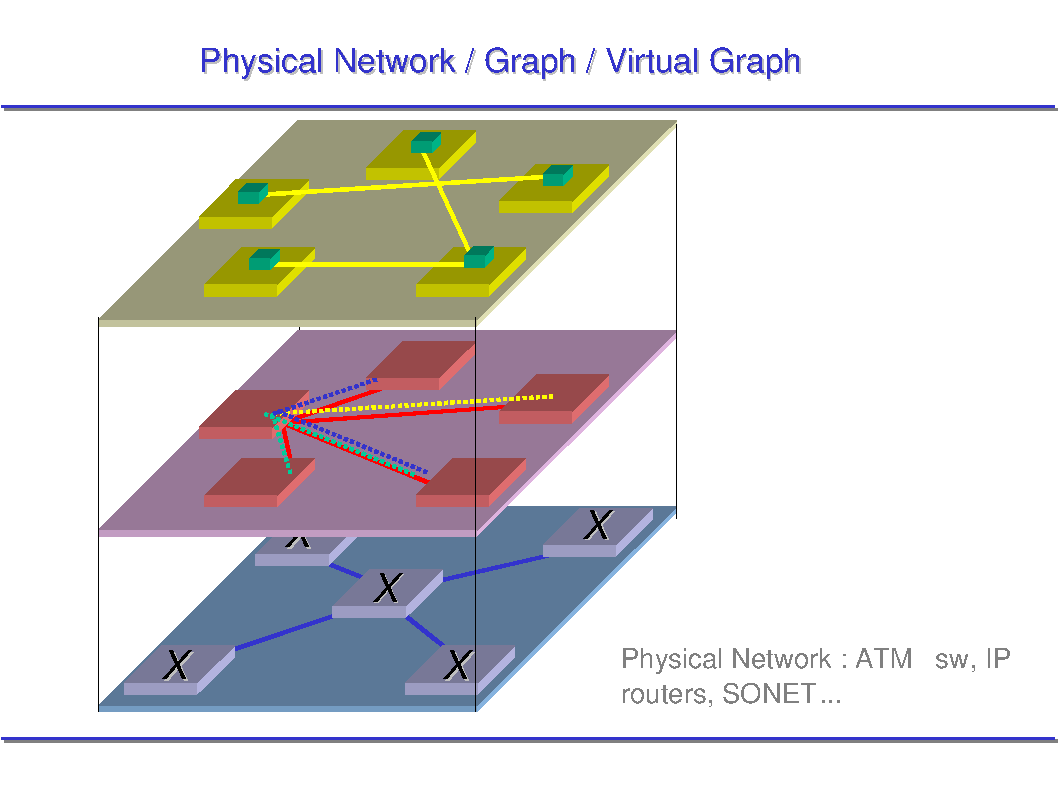
\includegraphics[scale=.75]{figures/sample}}}
\caption{{{A pdf/eps fig }}}
\label{figureeps}
\end{center}
\end{figure}




\noindent{\bf The subfig package !!!!!!} \\ 
\label{id2718562}
 jsdlkfj lsjd jsdkfjlksdfj lkjdsf lj sdlfj lksdj fljdslk jlksdjf lkjdsf ljsdlk fj
dsfkjsd lkfjklsdjf lkjs dfj lkjsd flkj sdlkj lkmjs dflkj sdlfj lmksjd flkj lksdjf 
dsfkjsd lkfjklsdjf lkjs dfj lkjsd flkj sdlkj lkmjs dflkj sdlfj lmksjd flkj lksdjf 
dsfkjsd lkfjklsdjf lkjs dfj lkjsd flkj sdlkj lkmjs dflkj sdlfj lmksjd flkj lksdjf 
dsfkjsd lkfjklsdjf lkjs dfj lkjsd flkj sdlkj lkmjs dflkj sdlfj lmksjd flkj lksdjf 
dsfkjsd lkfjklsdjf lkjs dfj lkjsd flkj sdlkj lkmjs dflkj sdlfj lmksjd flkj lksdjf 
sdflj lkjsdf mklj sdkfklj jdsfklj dsflj sdfjklsjd lkj sdklj lkjlk jsdlfj lksj flj 
dsfkjsd lkfjklsdjf lkjs dfj lkjsd flkj sdlkj lkmjs dflkj sdlfj lmksjd flkj lksdjf 
dsfkjsd lkfjklsdjf lkjs dfj lkjsd flkj sdlkj lkmjs dflkj sdlfj lmksjd flkj lksdjf 
sdflj lkjsdf mklj sdkfklj jdsfklj dsflj sdfjklsjd lkj sdklj lkjlk jsdlfj lksj flj 
dsfkjsd lkfjklsdjf lkjs dfj lkjsd flkj sdlkj lkmjs dflkj sdlfj lmksjd flkj lksdjf 
sdflj lkjsdf mklj sdkfklj jdsfklj dsflj sdfjklsjd lkj sdklj lkjlk jsdlfj lksj flj 
sdflj lkjsdf mklj sdkfklj jdsfklj dsflj sdfjklsjd lkj sdklj lkjlk jsdlfj lksj flj 
dsfkjsd lkfjklsdjf lkjs dfj lkjsd flkj sdlkj lkmjs dflkj sdlfj lmksjd flkj lksdjf 
sdflj lkjsdf mklj sdkfklj jdsfklj dsflj sdfjklsjd lkj sdklj lkjlk jsdlfj lksj flj 
dsfkjsd lkfjklsdjf lkjs dfj lkjsd flkj sdlkj lkmjs dflkj sdlfj lmksjd flkj lksdjf 
sdflj lkjsdf mklj sdkfklj jdsfklj dsflj sdfjklsjd lkj sdklj lkjlk jsdlfj lksj flj 
sdflj lkjsdf mklj sdkfklj jdsfklj dsflj sdfjklsjd lkj sdklj lkjlk jsdlfj lksj flj 
sdflj lkjsdf mklj sdkfklj jdsfklj dsflj sdfjklsjd lkj sdklj lkjlk jsdlfj lksj flj 
sdflj lkjsdf mklj sdkfklj jdsfklj dsflj sdfjklsjd lkj sdklj lkjlk jsdlfj lksj flj 
sdflj lkjsdf mklj sdkfklj jdsfklj dsflj sdfjklsjd lkj sdklj lkjlk jsdlfj lksj flj 


% figure ------------------------------------------------------
\begin{figure}[hbt]
\begin{center}%
\hypertarget{fig}{}%

{\subfigure[]{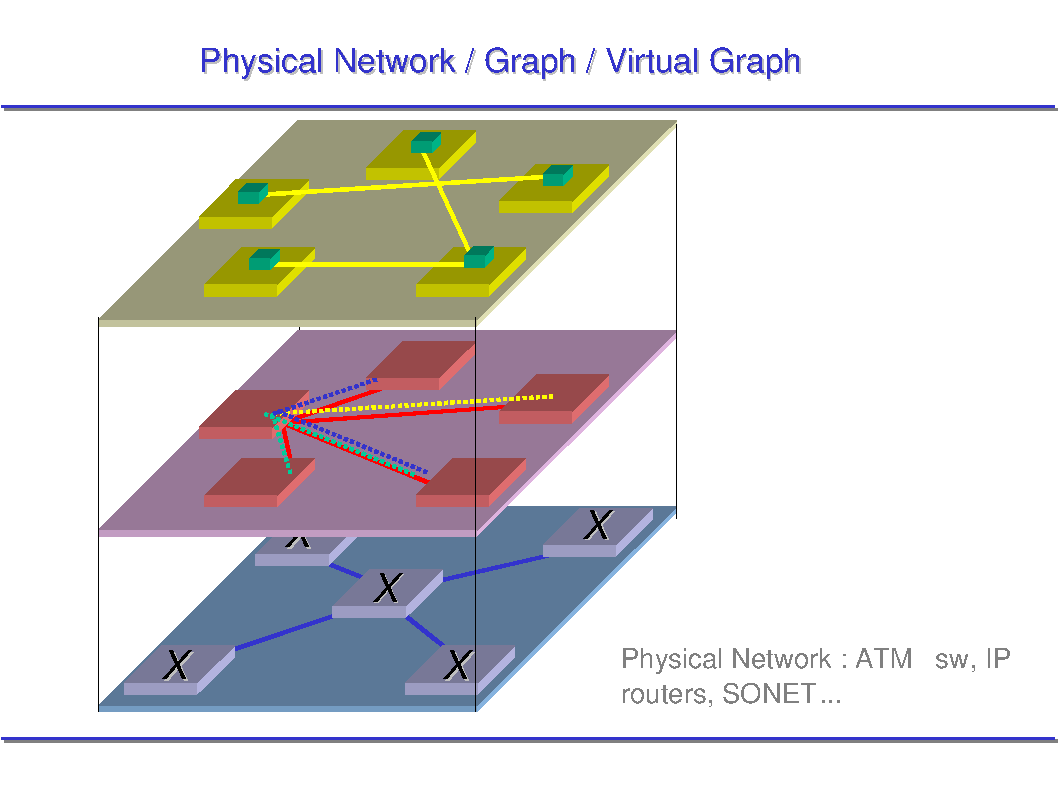
\includegraphics[scale=.40]{figures/sample}}}
\caption{{{ LOOK WHAT HAPPENS WHEN YOU PUT SEVERAL IMAGEOBJECT !!! }}}
\label{fig}
\end{center}
\end{figure}




\noindent{\bf Equation} \\ 
\label{id2780676}
\begin{dbequation}
\begin{center}

\includegraphics{figures/eq}
    \caption{An Equation}
\label{equation}\hypertarget{equation}{}%
\end{center}
\end{dbequation}




\noindent{\bf Table} \\ 
\label{id2780703}
% table ------------------------------------------------------
\begin{table}[hbt]
\begin{center}%
\hypertarget{table}{}%
\captionswapskip{}\caption{A Table}
\captionswapskip{}\begin{tabular}{|c|c|}
\hline 
1\%1 & 1 \tabularnewline
 \hline 
2 & 4 \tabularnewline
 \hline 
3 & 9 \tabularnewline
\hline 
\end{tabular}
\label{table}
\end{center}
\end{table}


% ------------------------   
% Section 
\section{Informal Objects}
\label{id2780781}\hypertarget{id2780781}{}%



\noindent{\bf InformalExample} \\ 
\label{id2780789}\label{iexample}
This is an example of a trivial, informal example.



\noindent{\bf InformalEquation} \\ 
\label{id2780809}\label{iequation}
\includegraphics{figures/eq}
    


\noindent{\bf InformalTable} \\ 
\label{id2780833}
% tabular ------------------------------------------------------
\begin{center}
\label{itable}\hypertarget{itable}{}%
\begin{tabular}{|c|c|}
\hline 
1 & 1 \tabularnewline
 \hline 
2 & 8 \tabularnewline
 \hline 
3 & 27 \tabularnewline
\hline 
\end{tabular}
\end{center}


% ------------------------   
% Section 
\section{Admonitions}
\label{id2780896}\hypertarget{id2780896}{}%



\noindent{\bf Note} \\ 
\label{id2780905}
\begin{admonition}{figures/note}{Note}% NOTICE: see the db2latex FAQ w.r.t db2latex variable $latex.admonition.path

Consider yourself noted.

Second para.
\end{admonition}


\begin{admonition}{figures/note}{Note}% NOTICE: see the db2latex FAQ w.r.t db2latex variable $latex.admonition.path

Consider yourself noted, simply.
\end{admonition}


\begin{admonition}{figures/note}{NoteTitle}% NOTICE: see the db2latex FAQ w.r.t db2latex variable $latex.admonition.path

Consider yourself noted.

Second para, with a title.
\end{admonition}


\begin{admonition}{figures/note}{Att}% NOTICE: see the db2latex FAQ w.r.t db2latex variable $latex.admonition.path

Consider yourself noted, simply.

With a title
\end{admonition}




\noindent{\bf Important} \\ 
\label{id2780967}
\begin{admonition}{figures/important}{Important}% NOTICE: see the db2latex FAQ w.r.t db2latex variable $latex.admonition.path

Consider yourself important.
\end{admonition}




\noindent{\bf Tip} \\ 
\label{id2780983}
\begin{admonition}{figures/tip}{Tip}% NOTICE: see the db2latex FAQ w.r.t db2latex variable $latex.admonition.path

Consider yourself tipped.
\end{admonition}




\noindent{\bf Warning} \\ 
\label{id2780998}
\begin{admonition}{figures/warning}{Warning}% NOTICE: see the db2latex FAQ w.r.t db2latex variable $latex.admonition.path

Consider yourself warned.
\end{admonition}




\noindent{\bf Caution} \\ 
\label{id2781013}
\begin{admonition}{figures/caution}{Caution}% NOTICE: see the db2latex FAQ w.r.t db2latex variable $latex.admonition.path

Consider yourself cautioned.
\end{admonition}




\noindent{\bf SimPara in Caution} \\ 
\label{id2781029}
\begin{admonition}{figures/caution}{Simple Caution}% NOTICE: see the db2latex FAQ w.r.t db2latex variable $latex.admonition.path

A simpler caution.
\end{admonition}


% ------------------------   
% Section 
\section{Other Objects}
\label{id2781049}\hypertarget{id2781049}{}%



\noindent{\bf Screen} \\ 
\label{id2781057}
\begin{Verbatim}[]
This
  is                  With a line-annotation
    a 
     screen
     This
    is                With a line-annotation
  a 
screen
This
  is                  With a line-annotation
    a 
     screen
\end{Verbatim}



\noindent{\bf ProgramListing} \\ 
\label{id2781087}
\begin{Verbatim}[]
This
  is
    a 
programlisting
\end{Verbatim}



\noindent{\bf Address} \\ 
\label{id2781102}
\begin{verbatim}
Norman Walsh
ArborText, Inc.
1000 Victors Way
Ann Arbor, MI 48108
US

Voice: 313.997.0200
Fax: 313.997.0201

Email: nwalsh@arbortext.com
WWW: http://www.arbortext.com/
\end{verbatim}



\noindent{\bf BlockQuote} \\ 
\label{id2781155}\begin{quote}
The universe that we observe has precisely the properties we should 
expect if there is, at bottom, no design, no purpose, no evil and
no good, nothing but pitiless indifference. -- Richard Dawkins
\end{quote}



\noindent{\bf Procedure} \\ 
\label{id2781174}\begin{enumerate}
\item{{This is the first step}}
\item{{This is the second step\begin{enumerate}
\item{{This is the first substep}}
\item{{This is the second substep}}
\end{enumerate}
}}
\item{{This is the third step}}
\end{enumerate}



\noindent{\bf Procedure With Title} \\ 
\label{id2781248}{\sc{Same Procedure with a Title}}
\begin{enumerate}
\item{{This is the first step}}
\item{{This is the second step\begin{enumerate}
\item{{This is the first substep}}
\item{{This is the second substep}}
\end{enumerate}
}}
\item{{This is the third step}}
\end{enumerate}



\noindent{\bf SideBar} \\ 
\label{id2781326}\label{id2781332}What About Bob?

This is a sidebar.



\noindent{\bf MsgSet} \\ 
\label{id2781346}
It's not really clear how {\tt{MsgSet}} should be presented.
I expect that it's fairly application, if not document, specific.
\label{id2781366}\label{id2781369}
Record failed CRC

Record {\tt\itshape{n}}
                    in {\tt\itshape{database}}

File read error on 
                   {\tt\itshape{database}}

Panic! Corrupt record!
\label{id2781434}Level: severeOrigin: serverAudience: all\label{id2781450}
        Indicates that some sort of error occured attempting to load
        a record from the database.  Retry.  If failure persists,
        contact the database administrator.
        



\noindent{\bf LiteralLayout} \\ 
\label{id2781466}
\begin{Verbatim}[,fontfamily=default]
This is a
literal
       layout
\end{Verbatim}


\begin{Verbatim}[,fontfamily=default]
This is a
literal
       layout
  in a para
\end{Verbatim}


% -------------------------------------------------------------
% Chapter List Tests 
% ------------------------------------------------------------- 	
\chapter{List Tests}
\label{id2781496}\hypertarget{id2781496}{}%

% ------------------------   
% Section 
\section{OrderedLists}
\label{id2781503}\hypertarget{id2781503}{}%

{\sc Font Filename Extensions}

\noindent
 
	\begin{description}
	\item[{\tt{TTF}}] 

TrueType fonts.

\item[{\tt{PFA}}, {\tt{PFB}}] 

PostScript fonts.  {\tt{PFA}} files are common on 
UNIX systems, {\tt{PFB}} files
are more common on Windows systems.


	\end{description}
    


\noindent{\bf Default Numeration} \\ 
\label{id2781587}\begin{enumerate}
	\item 
One


	\item 
\begin{Verbatim}[]
this one starts with
a program listing
what happens?
\end{Verbatim}


	\item \label{id2781625}this one starts with
a synopsis
what happens?

	\item 
para first
\label{id2781640}this one has
a synopsis
what happens?

	\item 
Three

\begin{Verbatim}[]
A
Screen
Here
\end{Verbatim}


	\item 
Four


	\end{enumerate}

    


\noindent{\bf Arabic Numeration} \\ 
\label{id2781675}\begin{enumerate}[1]
	\item 
One


	\item 
Two


	\item 
Three


	\item 
Four


	\end{enumerate}

    


\noindent{\bf Arabic Numeration (Long)} \\ 
\label{id2781727}\begin{enumerate}[1]
	\item 
One


	\item 
Two


	\item 
Three


	\item 
Four


	\item 
Five


	\item 
Six


	\item 
Seven


	\item 
Eight


	\item 
Nine


	\item 
Ten


	\item 
Eleven


	\end{enumerate}

    


\noindent{\bf UpperAlpha Numeration} \\ 
\label{id2781838}\begin{enumerate}[A]
	\item 
One


	\item 
Two


	\item 
Three


	\item 
Four


	\end{enumerate}

    


\noindent{\bf LowerAlpha Numeration} \\ 
\label{id2781891}\begin{enumerate}[a]
	\item 
One


	\item 
Two


	\item 
Three


	\item 
Four


	\end{enumerate}

    


\noindent{\bf UpperRoman Numeration} \\ 
\label{id2781943}\begin{enumerate}[I]
	\item 
One


	\item 
Two


	\item 
Three


	\item 
Four


	\end{enumerate}

    


\noindent{\bf LowerRoman Numeration} \\ 
\label{id2781995}\begin{enumerate}[i]
	\item 
One


	\item 
Two


	\item 
Three


	\item 
Four


	\end{enumerate}

    


\noindent{\bf Continued} \\ 
\label{id2782048}
First list:
\begin{enumerate}
	\item 
One


	\item 
Two


	\item 
Three


	\item 
Four


	\end{enumerate}

    

Second list:
\begin{enumerate}
	\item 
Five


	\item 
Six


	\item 
Seven


	\item 
Eight


	\item 
Nine


	\item 
Ten


	\end{enumerate}

    

% ------------------------   
% Section 
\section{ItemizedLists}
\label{id2782162}\hypertarget{id2782162}{}%



\noindent{\bf Default Presentation} \\ 
\label{id2782171}\begin{itemize}

	\item 
One


	\item 
\begin{Verbatim}[]
One-point-five. This one starts with
a program listing
what happens?
\end{Verbatim}


	\item 
Two


	\item 
Three


	\item 
Four

\end{itemize}



\noindent{\bf Block Elements in a List} \\ 
\label{id2782229}\begin{itemize}

	\item 
One

Another para.


	\item 
Two


	\item 
Three


	\item 
Four

\end{itemize}



\noindent{\bf Alternate Mark and OverRide} \\ 
\label{id2782278}\begin{itemize}

	\item 
TeX and LaTeX


	\item 
Troff


	\item 
Lout


	\item 
Test

\end{itemize}



\noindent{\bf No mark Presentation} \\ 
\label{id2782330}\begin{itemize}

	\item 
One


	\item 
Two


	\item 
Three


	\item 
Four

\end{itemize}

% ------------------------   
% Section 
\section{VariableLists}
\label{id2782382}\hypertarget{id2782382}{}%

\noindent
 
	\begin{description}
	\item[Term1] 
Blah blah blah blah. Blah blah blah blah. Blah blah blah blah.
Blah blah blah blah. Blah blah blah blah. Blah blah blah blah.
Blah blah blah blah. Blah blah blah blah. Blah blah blah blah.
Blah blah blah blah. Blah blah blah blah. Blah blah blah blah.
Blah blah blah blah. Blah blah blah blah. Blah blah blah blah.
\item[Term2] 
Blah blah blah blah. Blah blah blah blah. Blah blah blah blah.
Blah blah blah blah. Blah blah blah blah. Blah blah blah blah.
Blah blah blah blah. Blah blah blah blah. Blah blah blah blah.
Blah blah blah blah. Blah blah blah blah. Blah blah blah blah.
Blah blah blah blah. Blah blah blah blah. Blah blah blah blah.
\item[Term3] 
Blah blah blah blah. Blah blah blah blah. Blah blah blah blah.
Blah blah blah blah. Blah blah blah blah. Blah blah blah blah.
Blah blah blah blah. Blah blah blah blah. Blah blah blah blah.
Blah blah blah blah. Blah blah blah blah. Blah blah blah blah.
Blah blah blah blah. Blah blah blah blah. Blah blah blah blah.
\begin{itemize}

	\item 
One


	\item 
Two


	\item 
Three


	\item 
Four

\end{itemize}

Blah blah blah blah. Blah blah blah blah. Blah blah blah blah.
Blah blah blah blah. Blah blah blah blah. Blah blah blah blah.
Blah blah blah blah. Blah blah blah blah. Blah blah blah blah.
Blah blah blah blah. Blah blah blah blah. Blah blah blah blah.
Blah blah blah blah. Blah blah blah blah. Blah blah blah blah.
\item[Term4] 
Blah blah blah blah. Blah blah blah blah. Blah blah blah blah.
Blah blah blah blah. Blah blah blah blah. Blah blah blah blah.
Blah blah blah blah. Blah blah blah blah. Blah blah blah blah.
Blah blah blah blah. Blah blah blah blah. Blah blah blah blah.
Blah blah blah blah. Blah blah blah blah. Blah blah blah blah.

	\end{description}
    
\noindent
 
	\begin{description}
	\item[Another List] 
Blah blah blah blah. Blah blah blah blah. Blah blah blah blah.
Blah blah blah blah. Blah blah blah blah. Blah blah blah blah.
Blah blah blah blah. Blah blah blah blah. Blah blah blah blah.
Blah blah blah blah. Blah blah blah blah. Blah blah blah blah.
Blah blah blah blah. Blah blah blah blah. Blah blah blah blah.
\item[ProgramListing] 
\begin{Verbatim}[]
A ProgramListing
Is the First Element
of this VarListEntry
\end{Verbatim}

Blah blah blah blah. Blah blah blah blah. Blah blah blah blah.
Blah blah blah blah. Blah blah blah blah. Blah blah blah blah.
Blah blah blah blah. Blah blah blah blah. Blah blah blah blah.
Blah blah blah blah. Blah blah blah blah. Blah blah blah blah.
Blah blah blah blah. Blah blah blah blah. Blah blah blah blah.

	\end{description}
    
% ------------------------   
% Section 
\section{SimpleLists}
\label{id2782592}\hypertarget{id2782592}{}%



\noindent{\bf Inline} \\ 
\label{id2782601}
An inline simple list:
One, Two, Three, Four, Five, Six, Seven



\noindent{\bf Horiz} \\ 
\label{id2782646}
\begin{tabular*}{\linewidth}{lll} 
One & Two & Three  \\
Four & Five & Six  \\
Seven &  \\
\end{tabular*}



\noindent{\bf Vert} \\ 
\label{id2782691}
\vspace{1cm}
\begin{tabular*}{\linewidth}{lll}
One & Four & Seven  \\
Two & Five &  \\
Three & Six &  \\
\end{tabular*}
\vspace{1cm}

% ------------------------   
% Section 
\section{More Complex List Item Content}
\label{id2782737}\hypertarget{id2782737}{}%
\begin{itemize}

	\item 
One

Second para


	\item 
Two

Second para


	\item 
Three

Second para


	\item 
Four

Second para


	\item 
{\bf Formal Element} 
Five



Second para


	\item 
Six

\end{itemize}
\begin{enumerate}
	\item 
One

Second para


	\item 
Two

Second para


	\item 
Three

Second para


	\item 
Four

Second para


	\item 
{\bf Formal Element} 
Five



Second para


	\item 
Six


	\end{enumerate}

    
% ------------------------   
% Section 
\section{Segmented List}
\label{id2782916}\hypertarget{id2782916}{}%

{\sc State Birds}

{ \em State:} Alabama{ \em Bird:} Yellowhammer \\
{ \em State:} Alaska{ \em Bird:} Willow Ptarmigan \\
{ \em State:} Arizona{ \em Bird:} Cactus Wren \\
{ \em State:} Arkansas{ \em Bird:} Mockingbird \\
{ \em State:} California{ \em Bird:} California Valley Quail \\
{ \em State:} Colorado{ \em Bird:} Lark Bunting \\
{ \em State:} Connecticut{ \em Bird:} Robin \\
{ \em State:} Delaware{ \em Bird:} Blue Hen Chicken \\
{ \em State:} Florida{ \em Bird:} Mockingbird \\
{ \em State:} Georgia{ \em Bird:} Brown Thrasher \\
{ \em State:} Hawaii{ \em Bird:} Nene \\
{ \em State:} Idaho{ \em Bird:} Mountain Bluebird \\
{ \em State:} Illinois{ \em Bird:} Cardinal \\
{ \em State:} Indiana{ \em Bird:} Cardinal \\
{ \em State:} Iowa{ \em Bird:} Eastern Goldfinch \\
{ \em State:} Kansas{ \em Bird:} Western Meadowlark \\
{ \em State:} Kentucky{ \em Bird:} Cardinal \\
{ \em State:} Louisiana{ \em Bird:} Eastern Brown Pelican \\
{ \em State:} Maine{ \em Bird:} Chickadee \\
{ \em State:} Maryland{ \em Bird:} Baltimore Oriole \\
{ \em State:} Massachusetts{ \em Bird:} Chickadee \\
{ \em State:} Michigan{ \em Bird:} Robin \\
{ \em State:} Minnesota{ \em Bird:} Common Loon \\
{ \em State:} Mississippi{ \em Bird:} Mockingbird \\
{ \em State:} Missouri{ \em Bird:} Bluebird \\
{ \em State:} Montana{ \em Bird:} Western Meadowlark \\
{ \em State:} Nebraska{ \em Bird:} Western Meadowlark \\
{ \em State:} Nevada{ \em Bird:} Mountain Bluebird \\
{ \em State:} New Hampshire{ \em Bird:} Purple Finch \\
{ \em State:} New Jersey{ \em Bird:} Eastern Goldfinch \\
{ \em State:} New Mexico{ \em Bird:} Roadrunner \\
{ \em State:} New York{ \em Bird:} Bluebird \\
{ \em State:} North Carolina{ \em Bird:} Cardinal \\
{ \em State:} North Dakota{ \em Bird:} Western Meadowlark \\
{ \em State:} Ohio{ \em Bird:} Cardinal \\
{ \em State:} Oklahoma{ \em Bird:} Scissor-tailed Flycatcher \\
{ \em State:} Oregon{ \em Bird:} Western Meadowlark \\
{ \em State:} Pennsylvania{ \em Bird:} Ruffed Grouse \\
{ \em State:} Rhode Island{ \em Bird:} Rhode Island Red \\
{ \em State:} South Carolina{ \em Bird:} Great Carolina Wren \\
{ \em State:} South Dakota{ \em Bird:} Ring-necked Pheasant \\
{ \em State:} Tennessee{ \em Bird:} Mockingbird \\
{ \em State:} Texas{ \em Bird:} Mockingbird \\
{ \em State:} Utah{ \em Bird:} American Seagull \\
{ \em State:} Vermont{ \em Bird:} Hermit Thrush \\
{ \em State:} Virginia{ \em Bird:} Cardinal  \\
{ \em State:} Washington{ \em Bird:} Willow Goldfinch \\
{ \em State:} West Virginia{ \em Bird:} Cardinal \\
{ \em State:} Wisconsin{ \em Bird:} Robin \\
{ \em State:} Wyoming{ \em Bird:} Western Meadowlark \\

% -------------------------------------------------------------
% Chapter Table Tests 
% ------------------------------------------------------------- 	
\chapter{Table Tests}
\label{id2783572}\hypertarget{id2783572}{}%



\noindent{\bf Alternate Alignment on Entry} \\ 
\label{id2783581}
% tabular ------------------------------------------------------
\begin{center}
\label{id2783589}\hypertarget{id2783589}{}%
\begin{tabular}{|p{2in}|p{2in}|c|}
\hline 
h1 & h2 & h3 \tabularnewline
 \hline 
\docbooktolatexalignll left\docbooktolatexalignlr  & \docbooktolatexaligncl center\docbooktolatexaligncr  & center \tabularnewline
 \hline 
\docbooktolatexaligncl center\docbooktolatexaligncr  & \docbooktolatexalignrl right\docbooktolatexalignrr  & \docbooktolatexalignrl right\docbooktolatexalignrr  \tabularnewline
\hline 
\end{tabular}
\end{center}


% tabular ------------------------------------------------------
\begin{center}
\label{id2783705}\hypertarget{id2783705}{}%
\begin{tabular}{p{2in}|p{2in}|c}
\hline 
h1 & h2 & h3 \tabularnewline
 \hline 
\docbooktolatexalignll left\docbooktolatexalignlr  & \docbooktolatexaligncl center\docbooktolatexaligncr  & center \tabularnewline
 \hline 
\docbooktolatexaligncl center\docbooktolatexaligncr  & \docbooktolatexalignrl right\docbooktolatexalignrr  & \docbooktolatexalignrl right\docbooktolatexalignrr  \tabularnewline
\hline 
\end{tabular}
\end{center}


% tabular ------------------------------------------------------
\begin{center}
\label{id2783822}\hypertarget{id2783822}{}%
\begin{tabular}{|p{2in}|p{2in}|c|}
\hline 
h1 & h2 & h3 \tabularnewline
 \hline 
\docbooktolatexalignll {\em left emph}\docbooktolatexalignlr  & \docbooktolatexaligncl {\bf center emph/bold}\docbooktolatexaligncr  & {\tt{center literal}} \tabularnewline
 \hline 
\docbooktolatexaligncl {\tt{center filename}}\docbooktolatexaligncr  & \docbooktolatexalignrl {\bf right command}\docbooktolatexalignrr  & \docbooktolatexalignrl right\docbooktolatexalignrr  \tabularnewline
\hline 
\end{tabular}
\end{center}




\noindent{\bf Absolute Widths} \\ 
\label{id2783954}
% tabular ------------------------------------------------------
\begin{center}
\label{id2783961}\hypertarget{id2783961}{}%
\begin{tabular}{|p{1in}|p{1in}|>{\Centering}p{1in}|}
\hline 
h1 & h2 & h3 \tabularnewline
 \hline 
e1 & e2 & e3 \tabularnewline
 \hline 
e1 & e2 & e3 \tabularnewline
 \hline 
e1 & e2 & e3 \tabularnewline
\hline 
\end{tabular}
\end{center}




\noindent{\bf Relative Widths} \\ 
\label{id2784082}
% tabular ------------------------------------------------------
\begin{center}
\label{id2784089}\hypertarget{id2784089}{}%
\begin{tabularx}{\columnwidth}{|>{\hsize=1.2\hsize}X|>{\hsize=0.8\hsize}X|}
\hline 
\docbooktolatexalignll left\docbooktolatexalignlr  & \docbooktolatexaligncl center\docbooktolatexaligncr  \tabularnewline
 \hline 
\docbooktolatexaligncl center\docbooktolatexaligncr  & \docbooktolatexalignrl right\docbooktolatexalignrr  \tabularnewline
\hline 
\end{tabularx}
\end{center}




\noindent{\bf Complex} \\ 
\label{id2784166}
% tabular ------------------------------------------------------
\begin{center}
\label{id2784172}\hypertarget{id2784172}{}%
\begin{tabular}{|c|r|c|c|c|c|}
\hline 
A1 & A2 & A3 & A4 & A5 & A6 \tabularnewline
 \hline 
B1 & B2 & B3 & B5 & B6 \tabularnewline
 \hline 
C1 & C2 & C3 & C4 & C5 \tabularnewline
 \hline 
D2 & D3 & D4 \tabularnewline
 \hline 
E1 & \docbooktolatexalignll E2\docbooktolatexalignlr  & E4 \tabularnewline
 \hline 
F1 & F2 & F3 & F4 & F5 & F6 \tabularnewline
\hline 
\end{tabular}
\end{center}




\noindent{\bf With Footnotes} \\ 
\label{id2784411}
% tabular ------------------------------------------------------
\begin{center}
\label{id2784418}\hypertarget{id2784418}{}%
\begin{minipage}{\linewidth}
\begin{tabular}{|c|c|}
\hline 
foo\label{fnrex1a}\begingroup\catcode`\#=12\footnote{A meaningless
word

}\endgroup\docbooktolatexmakefootnoteref{fnrex1a} & 3\label{fnrex1b}\begingroup\catcode`\#=12\footnote{A meaningless
number

}\endgroup\docbooktolatexmakefootnoteref{fnrex1b} \tabularnewline
 \hline 
bar\docbooktolatexusefootnoteref{fnrex1a} & 5\docbooktolatexusefootnoteref{fnrex1b} \tabularnewline
\hline 
\end{tabular}
\end{minipage}
\end{center}




\noindent{\bf A Big One} \\ 
\label{id2784491}
% tabular ------------------------------------------------------
\begin{center}
\label{id2784498}\hypertarget{id2784498}{}%
\begin{tabular}{|c|c|c|c|c|c|c|c|c|c|c|c|c|c|c|}
\hline 
H1 & H2 & H3 & H4 & H5 & H6 & H7 & H8 & H9 & H10 & H11 & H12 & H13 & H14 & H15 \tabularnewline
 \hline 
1 & 2 & 3 & 4 & 5 & 6 & 7 & 8 & 9 & 10 & 11 & 12 & 13 & 14 & 15 \tabularnewline
 \hline 
1 & 2 & 3 & 4 & 5 & 6 & 7 & 8 & 9 & 10 & 11 & 12 & 13 & 14 & 15 \tabularnewline
 \hline 
1 & 2 & 3 & 4 & 5 & 6 & 7 & 8 & 9 & 10 & 11 & 12 & 13 & 14 & 15 \tabularnewline
 \hline 
1 & 2 & 3 & 4 & 5 & 6 & 7 & 8 & 9 & 10 & 11 & 12 & 13 & 14 & 15 \tabularnewline
 \hline 
1 & 2 & 3 & 4 & 5 & 6 & 7 & 8 & 9 & 10 & 11 & 12 & 13 & 14 & 15 \tabularnewline
 \hline 
1 & 2 & 3 & 4 & 5 & 6 & 7 & 8 & 9 & 10 & 11 & 12 & 13 & 14 & 15 \tabularnewline
 \hline 
1 & 2 & 3 & 4 & 5 & 6 & 7 & 8 & 9 & 10 & 11 & 12 & 13 & 14 & 15 \tabularnewline
 \hline 
1 & 2 & 3 & 4 & 5 & 6 & 7 & 8 & 9 & 10 & 11 & 12 & 13 & 14 & 15 \tabularnewline
 \hline 
1 & 2 & 3 & 4 & 5 & 6 & 7 & 8 & 9 & 10 & 11 & 12 & 13 & 14 & 15 \tabularnewline
 \hline 
1 & 2 & 3 & 4 & 5 & 6 & 7 & 8 & 9 & 10 & 11 & 12 & 13 & 14 & 15 \tabularnewline
 \hline 
1 & 2 & 3 & 4 & 5 & 6 & 7 & 8 & 9 & 10 & 11 & 12 & 13 & 14 & 15 \tabularnewline
 \hline 
1 & 2 & 3 & 4 & 5 & 6 & 7 & 8 & 9 & 10 & 11 & 12 & 13 & 14 & 15 \tabularnewline
 \hline 
1 & 2 & 3 & 4 & 5 & 6 & 7 & 8 & 9 & 10 & 11 & 12 & 13 & 14 & 15 \tabularnewline
 \hline 
1 & 2 & 3 & 4 & 5 & 6 & 7 & 8 & 9 & 10 & 11 & 12 & 13 & 14 & 15 \tabularnewline
 \hline 
1 & 2 & 3 & 4 & 5 & 6 & 7 & 8 & 9 & 10 & 11 & 12 & 13 & 14 & 15 \tabularnewline
 \hline 
1 & 2 & 3 & 4 & 5 & 6 & 7 & 8 & 9 & 10 & 11 & 12 & 13 & 14 & 15 \tabularnewline
 \hline 
1 & 2 & 3 & 4 & 5 & 6 & 7 & 8 & 9 & 10 & 11 & 12 & 13 & 14 & 15 \tabularnewline
 \hline 
1 & 2 & 3 & 4 & 5 & 6 & 7 & 8 & 9 & 10 & 11 & 12 & 13 & 14 & 15 \tabularnewline
 \hline 
1 & 2 & 3 & 4 & 5 & 6 & 7 & 8 & 9 & 10 & 11 & 12 & 13 & 14 & 15 \tabularnewline
 \hline 
1 & 2 & 3 & 4 & 5 & 6 & 7 & 8 & 9 & 10 & 11 & 12 & 13 & 14 & 15 \tabularnewline
 \hline 
1 & 2 & 3 & 4 & 5 & 6 & 7 & 8 & 9 & 10 & 11 & 12 & 13 & 14 & 15 \tabularnewline
 \hline 
1 & 2 & 3 & 4 & 5 & 6 & 7 & 8 & 9 & 10 & 11 & 12 & 13 & 14 & 15 \tabularnewline
 \hline 
1 & 2 & 3 & 4 & 5 & 6 & 7 & 8 & 9 & 10 & 11 & 12 & 13 & 14 & 15 \tabularnewline
 \hline 
1 & 2 & 3 & 4 & 5 & 6 & 7 & 8 & 9 & 10 & 11 & 12 & 13 & 14 & 15 \tabularnewline
 \hline 
1 & 2 & 3 & 4 & 5 & 6 & 7 & 8 & 9 & 10 & 11 & 12 & 13 & 14 & 15 \tabularnewline
 \hline 
1 & 2 & 3 & 4 & 5 & 6 & 7 & 8 & 9 & 10 & 11 & 12 & 13 & 14 & 15 \tabularnewline
 \hline 
1 & 2 & 3 & 4 & 5 & 6 & 7 & 8 & 9 & 10 & 11 & 12 & 13 & 14 & 15 \tabularnewline
 \hline 
1 & 2 & 3 & 4 & 5 & 6 & 7 & 8 & 9 & 10 & 11 & 12 & 13 & 14 & 15 \tabularnewline
 \hline 
1 & 2 & 3 & 4 & 5 & 6 & 7 & 8 & 9 & 10 & 11 & 12 & 13 & 14 & 15 \tabularnewline
 \hline 
1 & 2 & 3 & 4 & 5 & 6 & 7 & 8 & 9 & 10 & 11 & 12 & 13 & 14 & 15 \tabularnewline
\hline 
\end{tabular}
\end{center}


% -------------------------------------------------------------
% Chapter Index Term Tests 
% ------------------------------------------------------------- 	
\chapter{Index Term Tests}
\label{id2786577}\hypertarget{id2786577}{}%

Test data.
\index{oft-repeated}\index{chap-level}
% ------------------------   
% Section 
\section{Index Term Sect 1}
\label{id2786619}\hypertarget{id2786619}{}%

Test data.
\index{!}\index{oft-repeated!with id}\index{sect1-level}\index{sect1-level}\index{sect1-level!sec}\index{sect1-other!sec}\index{chap-level!sec!tert}\index{chap-level!sec!tert}\index{sect1-level}\subsection{Index Term Sect 2}
\label{id2786792}\hypertarget{id2786792}{}%

Test data.
\index{[}\index{oft-repeated}\index{sect2-level}\index{chap-level!sec!tert}\subsection{Index Term Sect 3}
\label{id2786874}\hypertarget{id2786874}{}%

foo
% ------------------------------------------------------------- 
% 
% PART Part Two Title
% 
% ------------------------------------------------------------- 
\part{Part Two Title}
\label{part}\hypertarget{part}{}%

% -------------------------------------------------------------
% Chapter CmdSynopsis Tests 
% ------------------------------------------------------------- 	
\chapter{CmdSynopsis Tests}
\label{id2786900}\hypertarget{id2786900}{}%



\noindent{\bf Very Simple CmdSynopsis} \\ 
\label{id2786908}\label{id2786915}
\begin{list}{}{\setlength{\itemindent}{-\leftmargin}\setlength{\parsep}{0mm}}
\item\raggedright\texttt{cd {{\itshape directory}}}
\end{list}



\noindent{\bf Simple CmdSynopsis} \\ 
\label{id2786940}\label{id2786946}
\begin{list}{}{\setlength{\itemindent}{-\leftmargin}\setlength{\parsep}{0mm}}
\item\raggedright\texttt{cal [-j] [-y] [month  [year]]}
\end{list}



\noindent{\bf Another Simple CmdSynopsis} \\ 
\label{id2786996}\label{id2787003}
\begin{list}{}{\setlength{\itemindent}{-\leftmargin}\setlength{\parsep}{0mm}}
\item\raggedright\texttt{chgrp [-R 
     [-H | -L | -P]
  ] [-f]  {\itshape group}   {\itshape file}... }
\end{list}



\noindent{\bf Slightly Complex CmdSynopsis} \\ 
\label{id2787095}\label{id2787102}
\begin{list}{}{\setlength{\itemindent}{-\leftmargin}\setlength{\parsep}{0mm}}
\item\raggedright\texttt{emacs [-t {\itshape file}] [-q] [-u {\itshape user}] [+{\itshape number}] [-f {\itshape function}...] [-l {\itshape file}...]  {\itshape file}... }
\end{list}



\noindent{\bf Quite Complex CmdSynopsis} \\ 
\label{id2787196}\label{id2787203}
\begin{list}{}{\setlength{\itemindent}{-\leftmargin}\setlength{\parsep}{0mm}}
\item\raggedright\texttt{cccp [-\$] [-C] [-D{\itshape name} [={\itshape definition}]...] [-dD] [-dM] [-I {\itshape directory}...] [-H] [-I-]
 [-imacros {\itshape file}...] [-include {\itshape file}...] [-lang-c | -lang-c++ | -lang-objc] [-lint]
 [-M | -MD | -MM | -MMD] [-nostdinc] [-P] [-pedantic] [-pedantic-errors] [-trigraphs] [-U{\itshape name}]
 [-undef] [-Wtrigraphs] [-Wcomment] [-Wall] [-Wtraditional] {{\itshape infile} | -} {{\itshape outfile} | -}}
\end{list}

% -------------------------------------------------------------
% Chapter FuncSynopsis Tests 
% ------------------------------------------------------------- 	
\chapter{FuncSynopsis Tests}
\label{id2787600}\hypertarget{id2787600}{}%



\noindent{\bf Two Simple Parameters} \\ 
\label{id2787609}\label{id2787616}int  {\bf max } ({\tt\itshape{int1}}, {\tt\itshape{int2}});
	\newline
	int {\tt\itshape{int1}};
	\newline
	int {\tt\itshape{int2}};


\noindent{\bf Variable Arguments} \\ 
\label{id2787654}\label{id2787661}
\begin{verbatim}
#include <varargs.h>
\end{verbatim}
int  {\bf max } ( ... );


\noindent{\bf Void} \\ 
\label{id2787695}\label{id2787700}int  {\bf rand } ();


\noindent{\bf Function Pointer Arguments} \\ 
\label{id2787720}\label{id2787727}void  {\bf qsort } ({\tt\itshape{dataptr}}, {\tt\itshape{left}}, {\tt\itshape{right}}, {\tt\itshape{(* comp)}});
	\newline
	void *{\tt\itshape{dataptr}}[];
	\newline
	int {\tt\itshape{left}};
	\newline
	int {\tt\itshape{right}};
	\newline
	int {\tt\itshape{(* comp)}}
      (void *, void *);
% -------------------------------------------------------------
% Chapter Callout Tests 
% ------------------------------------------------------------- 	
\chapter{Callout Tests}
\label{id2787790}\hypertarget{id2787790}{}%



\noindent{\bf CallOut (using AREASPEC)} \\ 
\label{id2787798}
\begin{Verbatim}[]
@rem = '--*-Perl-*--
@echo off
perl.exe %_batchname %$
goto endofperl
@rem ';

# Compress mail...

require 'n:/home/nwalsh/lib/cygnus.pl';
require 'timelocal.pl';
use Cwd;

select (STDERR); $| = 1;
select (STDOUT); $| = 1;

@DIRS = ("/home/nwalsh/Mail");
while (@DIRS) {
    $dir = shift @DIRS;
    opendir (DIR, $dir);
    while ($fname = readdir(DIR)) {
        $file = "$dir/$fname";
        next if ! -d $file;
        next if $fname =~ /^\.\.?$/;

        print "$file\n";
        push (@DIRS, $file);
        &compress ($file);
    }
}

exit;
\end{Verbatim}
callout ???
The prologue handles embedding a Perl script in a DOS batch file.
callout ???
The {\tt{goto}} statement, interpreted by the DOS batch
file interpreter, skips over the body of the Perl script.
callout ???
The {\tt{require}} statement sources in external program
fragments.
callout ???
The {\tt{use}} statement is similar, but has additional
utility.  It is a Perl5 function.  (Note that this callout area specifies
both a line and a column.)
callout ???
This is a user subroutine call.



\noindent{\bf CallOut (using CO)} \\ 
\label{id2787995}
\begin{Verbatim}[]
this is a line
this is another line
there's a callout in here.
and there's another on the
next line
right here:
\end{Verbatim}
\href{ callout1}{callout1} 
First callout.

Second para in first callout.
\href{ callout2}{callout2} 
Blah blah blah blah. Blah blah blah blah. Blah blah blah blah.
Blah blah blah blah. Blah blah blah blah. Blah blah blah blah.
Blah blah blah blah. Blah blah blah blah. Blah blah blah blah.
Blah blah blah blah. Blah blah blah blah. Blah blah blah blah.
Blah blah blah blah. Blah blah blah blah. Blah blah blah blah.

Second callout.

Third para in second callout.
\href{ callout1}{callout1} \href{ callout2}{callout2} 
This paragraph describes {\em both} callouts.
% ------------------------------------------------------------- 
% 
% PART A Reference Part
% 
% ------------------------------------------------------------- 
\part{A Reference Part}
\label{id2788089}\hypertarget{id2788089}{}%
% 
% -------------------------------------------------------------
% Reference 
% ------------------------------------------------------------- 	
\chapter*{Reference}
\label{reference}\hypertarget{reference}{}%
% 
% -------------------------------------------------------------
% Refentry 
% ------------------------------------------------------------- 	
\section*{RefEntryTitle}
\label{id2788106}\hypertarget{id2788106}{}%
\label{id2788118}RefName1
\subsection*{Name}
RefName1, RefName2RefName2 $-$ Yes, there must be a purpose!\label{id2788140}
\subsection*{Synopsis}
\label{id2788143}  A
   Synopsis
    Goes
   Here
\subsection*{A RefSect1}
\label{id2788151}

Blah blah blah blah. Blah blah blah blah. Blah blah blah blah.
Blah blah blah blah. Blah blah blah blah. Blah blah blah blah.
Blah blah blah blah. Blah blah blah blah. Blah blah blah blah.
Blah blah blah blah. Blah blah blah blah. Blah blah blah blah.
Blah blah blah blah. Blah blah blah blah. Blah blah blah blah.

\subsubsection*{A RefSect2}
\label{id2788168}

Blah blah blah blah. Blah blah blah blah. Blah blah blah blah.
Blah blah blah blah. Blah blah blah blah. Blah blah blah blah.
Blah blah blah blah. Blah blah blah blah. Blah blah blah blah.
Blah blah blah blah. Blah blah blah blah. Blah blah blah blah.
Blah blah blah blah. Blah blah blah blah. Blah blah blah blah.

\paragraph*{A RefSect3}
\label{id2788185}

Blah blah blah blah. Blah blah blah blah. Blah blah blah blah.
Blah blah blah blah. Blah blah blah blah. Blah blah blah blah.
Blah blah blah blah.\label{id2788197}\begingroup\catcode`\#=12\footnote{This is a footnote in a refentry.

}\endgroup\docbooktolatexmakefootnoteref{id2788197}
Blah blah blah blah. Blah blah blah blah.
Blah blah blah blah. Blah blah blah blah. Blah blah blah blah.
Blah blah blah blah. Blah blah blah blah. Blah blah blah blah.
% 
% -------------------------------------------------------------
% Refentry 
% ------------------------------------------------------------- 	
\section*{{\tt{Chop}}}
\label{id2788214}\hypertarget{id2788214}{}%
\label{id2788217}{\tt{Chop}}
\subsection*{Name}
{\tt{Chop}} $-$ strip trailing whitespace
\subsection*{Description}
\label{id2788234}

     Returns the argument string without trailing whitespace.
     
\begin{example}%
\captionswapskip{}\caption{chop() example}
\captionswapskip{}
\begin{Verbatim}[]
$trimmed = Chop($line);
\end{Verbatim}
\label{id2788245}\hypertarget{id2788245}{}%
\end{example}


    

\newcommand{\dbappendix}[1]{\chapter{#1}}%
% ------------------------------------------------------------- 
% Appendixes start here
% -------------------------------------------------------------
\appendix

% -------------------------------------------------------------
% appendix:  A Very Short Appendix 
% ------------------------------------------------------------- 	
\dbappendix{A Very Short Appendix}
\label{appendix}\hypertarget{appendix}{}%

Blah.

% -------------------------------------------------------------
% appendix:  A Very Long Appendix 
% ------------------------------------------------------------- 	
\dbappendix{A Very Long Appendix}
\label{id2788284}\hypertarget{id2788284}{}%

Blah blah blah blah. Blah blah blah blah. Blah blah blah blah.
Blah blah blah blah. Blah blah blah blah. Blah blah blah blah.
Blah blah blah blah. Blah blah blah blah. Blah blah blah blah.
Blah blah blah blah. Blah blah blah blah. Blah blah blah blah.
Blah blah blah blah. Blah blah blah blah. Blah blah blah blah.

Blah blah blah blah. Blah blah blah blah. Blah blah blah blah.
Blah blah blah blah. Blah blah blah blah. Blah blah blah blah.
Blah blah blah blah. Blah blah blah blah. Blah blah blah blah.
Blah blah blah blah. Blah blah blah blah. Blah blah blah blah.
Blah blah blah blah. Blah blah blah blah. Blah blah blah blah.

Blah blah blah blah. Blah blah blah blah. Blah blah blah blah.
Blah blah blah blah. Blah blah blah blah. Blah blah blah blah.
Blah blah blah blah. Blah blah blah blah. Blah blah blah blah.
Blah blah blah blah. Blah blah blah blah. Blah blah blah blah.
Blah blah blah blah. Blah blah blah blah. Blah blah blah blah.

Blah blah blah blah. Blah blah blah blah. Blah blah blah blah.
Blah blah blah blah. Blah blah blah blah. Blah blah blah blah.
Blah blah blah blah. Blah blah blah blah. Blah blah blah blah.
Blah blah blah blah. Blah blah blah blah. Blah blah blah blah.
Blah blah blah blah. Blah blah blah blah. Blah blah blah blah.

Blah blah blah blah. Blah blah blah blah. Blah blah blah blah.
Blah blah blah blah. Blah blah blah blah. Blah blah blah blah.
Blah blah blah blah. Blah blah blah blah. Blah blah blah blah.
Blah blah blah blah. Blah blah blah blah. Blah blah blah blah.
Blah blah blah blah. Blah blah blah blah. Blah blah blah blah.

Blah blah blah blah. Blah blah blah blah. Blah blah blah blah.
Blah blah blah blah. Blah blah blah blah. Blah blah blah blah.
Blah blah blah blah. Blah blah blah blah. Blah blah blah blah.
Blah blah blah blah. Blah blah blah blah. Blah blah blah blah.
Blah blah blah blah. Blah blah blah blah. Blah blah blah blah.

Blah blah blah blah. Blah blah blah blah. Blah blah blah blah.
Blah blah blah blah. Blah blah blah blah. Blah blah blah blah.
Blah blah blah blah. Blah blah blah blah. Blah blah blah blah.
Blah blah blah blah. Blah blah blah blah. Blah blah blah blah.
Blah blah blah blah. Blah blah blah blah. Blah blah blah blah.

Blah blah blah blah. Blah blah blah blah. Blah blah blah blah.
Blah blah blah blah. Blah blah blah blah. Blah blah blah blah.
Blah blah blah blah. Blah blah blah blah. Blah blah blah blah.
Blah blah blah blah. Blah blah blah blah. Blah blah blah blah.
Blah blah blah blah. Blah blah blah blah. Blah blah blah blah.

Blah blah blah blah. Blah blah blah blah. Blah blah blah blah.
Blah blah blah blah. Blah blah blah blah. Blah blah blah blah.
Blah blah blah blah. Blah blah blah blah. Blah blah blah blah.
Blah blah blah blah. Blah blah blah blah. Blah blah blah blah.
Blah blah blah blah. Blah blah blah blah. Blah blah blah blah.

Blah blah blah blah. Blah blah blah blah. Blah blah blah blah.
Blah blah blah blah. Blah blah blah blah. Blah blah blah blah.
Blah blah blah blah. Blah blah blah blah. Blah blah blah blah.
Blah blah blah blah. Blah blah blah blah. Blah blah blah blah.
Blah blah blah blah. Blah blah blah blah. Blah blah blah blah.

Blah blah blah blah. Blah blah blah blah. Blah blah blah blah.
Blah blah blah blah. Blah blah blah blah. Blah blah blah blah.
Blah blah blah blah. Blah blah blah blah. Blah blah blah blah.
Blah blah blah blah. Blah blah blah blah. Blah blah blah blah.
Blah blah blah blah. Blah blah blah blah. Blah blah blah blah.

Blah blah blah blah. Blah blah blah blah. Blah blah blah blah.
Blah blah blah blah. Blah blah blah blah. Blah blah blah blah.
Blah blah blah blah. Blah blah blah blah. Blah blah blah blah.
Blah blah blah blah. Blah blah blah blah. Blah blah blah blah.
Blah blah blah blah. Blah blah blah blah. Blah blah blah blah.

Blah blah blah blah. Blah blah blah blah. Blah blah blah blah.
Blah blah blah blah. Blah blah blah blah. Blah blah blah blah.
Blah blah blah blah. Blah blah blah blah. Blah blah blah blah.
Blah blah blah blah. Blah blah blah blah. Blah blah blah blah.
Blah blah blah blah. Blah blah blah blah. Blah blah blah blah.

Blah blah blah blah. Blah blah blah blah. Blah blah blah blah.
Blah blah blah blah. Blah blah blah blah. Blah blah blah blah.
Blah blah blah blah. Blah blah blah blah. Blah blah blah blah.
Blah blah blah blah. Blah blah blah blah. Blah blah blah blah.
Blah blah blah blah. Blah blah blah blah. Blah blah blah blah.

Blah blah blah blah. Blah blah blah blah. Blah blah blah blah.
Blah blah blah blah. Blah blah blah blah. Blah blah blah blah.
Blah blah blah blah. Blah blah blah blah. Blah blah blah blah.
Blah blah blah blah. Blah blah blah blah. Blah blah blah blah.
Blah blah blah blah. Blah blah blah blah. Blah blah blah blah.

Blah blah blah blah. Blah blah blah blah. Blah blah blah blah.
Blah blah blah blah. Blah blah blah blah. Blah blah blah blah.
Blah blah blah blah. Blah blah blah blah. Blah blah blah blah.
Blah blah blah blah. Blah blah blah blah. Blah blah blah blah.
Blah blah blah blah. Blah blah blah blah. Blah blah blah blah.

Blah blah blah blah. Blah blah blah blah. Blah blah blah blah.
Blah blah blah blah. Blah blah blah blah. Blah blah blah blah.
Blah blah blah blah. Blah blah blah blah. Blah blah blah blah.
Blah blah blah blah. Blah blah blah blah. Blah blah blah blah.
Blah blah blah blah. Blah blah blah blah. Blah blah blah blah.

Blah blah blah blah. Blah blah blah blah. Blah blah blah blah.
Blah blah blah blah. Blah blah blah blah. Blah blah blah blah.
Blah blah blah blah. Blah blah blah blah. Blah blah blah blah.
Blah blah blah blah. Blah blah blah blah. Blah blah blah blah.
Blah blah blah blah. Blah blah blah blah. Blah blah blah blah.

Blah blah blah blah. Blah blah blah blah. Blah blah blah blah.
Blah blah blah blah. Blah blah blah blah. Blah blah blah blah.
Blah blah blah blah. Blah blah blah blah. Blah blah blah blah.
Blah blah blah blah. Blah blah blah blah. Blah blah blah blah.
Blah blah blah blah. Blah blah blah blah. Blah blah blah blah.

Blah blah blah blah. Blah blah blah blah. Blah blah blah blah.
Blah blah blah blah. Blah blah blah blah. Blah blah blah blah.
Blah blah blah blah. Blah blah blah blah. Blah blah blah blah.
Blah blah blah blah. Blah blah blah blah. Blah blah blah blah.
Blah blah blah blah. Blah blah blah blah. Blah blah blah blah.

Blah blah blah blah. Blah blah blah blah. Blah blah blah blah.
Blah blah blah blah. Blah blah blah blah. Blah blah blah blah.
Blah blah blah blah. Blah blah blah blah. Blah blah blah blah.
Blah blah blah blah. Blah blah blah blah. Blah blah blah blah.
Blah blah blah blah. Blah blah blah blah. Blah blah blah blah.

Blah blah blah blah. Blah blah blah blah. Blah blah blah blah.
Blah blah blah blah. Blah blah blah blah. Blah blah blah blah.
Blah blah blah blah. Blah blah blah blah. Blah blah blah blah.
Blah blah blah blah. Blah blah blah blah. Blah blah blah blah.
Blah blah blah blah. Blah blah blah blah. Blah blah blah blah.

Blah blah blah blah. Blah blah blah blah. Blah blah blah blah.
Blah blah blah blah. Blah blah blah blah. Blah blah blah blah.
Blah blah blah blah. Blah blah blah blah. Blah blah blah blah.
Blah blah blah blah. Blah blah blah blah. Blah blah blah blah.
Blah blah blah blah. Blah blah blah blah. Blah blah blah blah.

Blah blah blah blah. Blah blah blah blah. Blah blah blah blah.
Blah blah blah blah. Blah blah blah blah. Blah blah blah blah.
Blah blah blah blah. Blah blah blah blah. Blah blah blah blah.
Blah blah blah blah. Blah blah blah blah. Blah blah blah blah.
Blah blah blah blah. Blah blah blah blah. Blah blah blah blah.

Blah blah blah blah. Blah blah blah blah. Blah blah blah blah.
Blah blah blah blah. Blah blah blah blah. Blah blah blah blah.
Blah blah blah blah. Blah blah blah blah. Blah blah blah blah.
Blah blah blah blah. Blah blah blah blah. Blah blah blah blah.
Blah blah blah blah. Blah blah blah blah. Blah blah blah blah.

Blah blah blah blah. Blah blah blah blah. Blah blah blah blah.
Blah blah blah blah. Blah blah blah blah. Blah blah blah blah.
Blah blah blah blah. Blah blah blah blah. Blah blah blah blah.
Blah blah blah blah. Blah blah blah blah. Blah blah blah blah.
Blah blah blah blah. Blah blah blah blah. Blah blah blah blah.

Blah blah blah blah. Blah blah blah blah. Blah blah blah blah.
Blah blah blah blah. Blah blah blah blah. Blah blah blah blah.
Blah blah blah blah. Blah blah blah blah. Blah blah blah blah.
Blah blah blah blah. Blah blah blah blah. Blah blah blah blah.
Blah blah blah blah. Blah blah blah blah. Blah blah blah blah.

Blah blah blah blah. Blah blah blah blah. Blah blah blah blah.
Blah blah blah blah. Blah blah blah blah. Blah blah blah blah.
Blah blah blah blah. Blah blah blah blah. Blah blah blah blah.
Blah blah blah blah. Blah blah blah blah. Blah blah blah blah.
Blah blah blah blah. Blah blah blah blah. Blah blah blah blah.

Blah blah blah blah. Blah blah blah blah. Blah blah blah blah.
Blah blah blah blah. Blah blah blah blah. Blah blah blah blah.
Blah blah blah blah. Blah blah blah blah. Blah blah blah blah.
Blah blah blah blah. Blah blah blah blah. Blah blah blah blah.
Blah blah blah blah. Blah blah blah blah. Blah blah blah blah.

Blah blah blah blah. Blah blah blah blah. Blah blah blah blah.
Blah blah blah blah. Blah blah blah blah. Blah blah blah blah.
Blah blah blah blah. Blah blah blah blah. Blah blah blah blah.
Blah blah blah blah. Blah blah blah blah. Blah blah blah blah.
Blah blah blah blah. Blah blah blah blah. Blah blah blah blah.

Blah blah blah blah. Blah blah blah blah. Blah blah blah blah.
Blah blah blah blah. Blah blah blah blah. Blah blah blah blah.
Blah blah blah blah. Blah blah blah blah. Blah blah blah blah.
Blah blah blah blah. Blah blah blah blah. Blah blah blah blah.
Blah blah blah blah. Blah blah blah blah. Blah blah blah blah.

Blah blah blah blah. Blah blah blah blah. Blah blah blah blah.
Blah blah blah blah. Blah blah blah blah. Blah blah blah blah.
Blah blah blah blah. Blah blah blah blah. Blah blah blah blah.
Blah blah blah blah. Blah blah blah blah. Blah blah blah blah.
Blah blah blah blah. Blah blah blah blah. Blah blah blah blah.

Blah blah blah blah. Blah blah blah blah. Blah blah blah blah.
Blah blah blah blah. Blah blah blah blah. Blah blah blah blah.
Blah blah blah blah. Blah blah blah blah. Blah blah blah blah.
Blah blah blah blah. Blah blah blah blah. Blah blah blah blah.
Blah blah blah blah. Blah blah blah blah. Blah blah blah blah.

Blah blah blah blah. Blah blah blah blah. Blah blah blah blah.
Blah blah blah blah. Blah blah blah blah. Blah blah blah blah.
Blah blah blah blah. Blah blah blah blah. Blah blah blah blah.
Blah blah blah blah. Blah blah blah blah. Blah blah blah blah.
Blah blah blah blah. Blah blah blah blah. Blah blah blah blah.

Blah blah blah blah. Blah blah blah blah. Blah blah blah blah.
Blah blah blah blah. Blah blah blah blah. Blah blah blah blah.
Blah blah blah blah. Blah blah blah blah. Blah blah blah blah.
Blah blah blah blah. Blah blah blah blah. Blah blah blah blah.
Blah blah blah blah. Blah blah blah blah. Blah blah blah blah.

Blah blah blah blah. Blah blah blah blah. Blah blah blah blah.
Blah blah blah blah. Blah blah blah blah. Blah blah blah blah.
Blah blah blah blah. Blah blah blah blah. Blah blah blah blah.
Blah blah blah blah. Blah blah blah blah. Blah blah blah blah.
Blah blah blah blah. Blah blah blah blah. Blah blah blah blah.

Blah blah blah blah. Blah blah blah blah. Blah blah blah blah.
Blah blah blah blah. Blah blah blah blah. Blah blah blah blah.
Blah blah blah blah. Blah blah blah blah. Blah blah blah blah.
Blah blah blah blah. Blah blah blah blah. Blah blah blah blah.
Blah blah blah blah. Blah blah blah blah. Blah blah blah blah.

Blah blah blah blah. Blah blah blah blah. Blah blah blah blah.
Blah blah blah blah. Blah blah blah blah. Blah blah blah blah.
Blah blah blah blah. Blah blah blah blah. Blah blah blah blah.
Blah blah blah blah. Blah blah blah blah. Blah blah blah blah.
Blah blah blah blah. Blah blah blah blah. Blah blah blah blah.

Blah blah blah blah. Blah blah blah blah. Blah blah blah blah.
Blah blah blah blah. Blah blah blah blah. Blah blah blah blah.
Blah blah blah blah. Blah blah blah blah. Blah blah blah blah.
Blah blah blah blah. Blah blah blah blah. Blah blah blah blah.
Blah blah blah blah. Blah blah blah blah. Blah blah blah blah.

Blah blah blah blah. Blah blah blah blah. Blah blah blah blah.
Blah blah blah blah. Blah blah blah blah. Blah blah blah blah.
Blah blah blah blah. Blah blah blah blah. Blah blah blah blah.
Blah blah blah blah. Blah blah blah blah. Blah blah blah blah.
Blah blah blah blah. Blah blah blah blah. Blah blah blah blah.

Blah blah blah blah. Blah blah blah blah. Blah blah blah blah.
Blah blah blah blah. Blah blah blah blah. Blah blah blah blah.
Blah blah blah blah. Blah blah blah blah. Blah blah blah blah.
Blah blah blah blah. Blah blah blah blah. Blah blah blah blah.
Blah blah blah blah. Blah blah blah blah. Blah blah blah blah.

Blah blah blah blah. Blah blah blah blah. Blah blah blah blah.
Blah blah blah blah. Blah blah blah blah. Blah blah blah blah.
Blah blah blah blah. Blah blah blah blah. Blah blah blah blah.
Blah blah blah blah. Blah blah blah blah. Blah blah blah blah.
Blah blah blah blah. Blah blah blah blah. Blah blah blah blah.

Blah blah blah blah. Blah blah blah blah. Blah blah blah blah.
Blah blah blah blah. Blah blah blah blah. Blah blah blah blah.
Blah blah blah blah. Blah blah blah blah. Blah blah blah blah.
Blah blah blah blah. Blah blah blah blah. Blah blah blah blah.
Blah blah blah blah. Blah blah blah blah. Blah blah blah blah.

Blah blah blah blah. Blah blah blah blah. Blah blah blah blah.
Blah blah blah blah. Blah blah blah blah. Blah blah blah blah.
Blah blah blah blah. Blah blah blah blah. Blah blah blah blah.
Blah blah blah blah. Blah blah blah blah. Blah blah blah blah.
Blah blah blah blah. Blah blah blah blah. Blah blah blah blah.

Blah blah blah blah. Blah blah blah blah. Blah blah blah blah.
Blah blah blah blah. Blah blah blah blah. Blah blah blah blah.
Blah blah blah blah. Blah blah blah blah. Blah blah blah blah.
Blah blah blah blah. Blah blah blah blah. Blah blah blah blah.
Blah blah blah blah. Blah blah blah blah. Blah blah blah blah.

Blah blah blah blah. Blah blah blah blah. Blah blah blah blah.
Blah blah blah blah. Blah blah blah blah. Blah blah blah blah.
Blah blah blah blah. Blah blah blah blah. Blah blah blah blah.
Blah blah blah blah. Blah blah blah blah. Blah blah blah blah.
Blah blah blah blah. Blah blah blah blah. Blah blah blah blah.

% ------------------------   
% Section 
\section{a sect1 title}
\label{id2788757}\hypertarget{id2788757}{}%

some text. some text. some text. some text. some text. some text. 
some text. some text. some text. some text. some text. some text. some text. 
some text. some text. some text. some text. some text. some text. some text. 
some text. some text. some text. some text. some text. some text. some text. 
some text. some text. some text. some text. some text. some text. some text. 
some text. some text. some text. some text. some text. some text. some text. 
\subsection{a sect2 title}
\label{id2788777}\hypertarget{id2788777}{}%

some text. some text. some text. some text. some text. some text. 
some text. some text. some text. some text. some text. some text. some text. 
some text. some text. some text. some text. some text. some text. some text. 
some text. some text. some text. some text. some text. some text. some text. 
some text. some text. some text. some text. some text. some text. some text. 
some text. some text. some text. some text. some text. some text. some text. 
\subsubsection{a sect3 title}
\label{id2788797}\hypertarget{id2788797}{}%

some text. some text. some text. some text. some text. some text. 
some text. some text. some text. some text. some text. some text. some text. 
some text. some text. some text. some text. some text. some text. some text. 
some text. some text. some text. some text. some text. some text. some text. 
some text. some text. some text. some text. some text. some text. some text. 
some text. some text. some text. some text. some text. some text. some text. 
\subparagraph*{a sect4 title}
\label{id2788818}\hypertarget{id2788818}{}%

some text. some text. some text. some text. some text. some text. 
some text. some text. some text. some text. some text. some text. some text. 
some text. some text. some text. some text. some text. some text. some text. 
some text. some text. some text. some text. some text. some text. some text. 
some text. some text. some text. some text. some text. some text. some text. 
some text. some text. some text. some text. some text. some text. some text. 
\subparagraph*{a sect5 title}
\label{id2788838}\hypertarget{id2788838}{}%

some text. some text. some text. some text. some text. some text. 
some text. some text. some text. some text. some text. some text. some text. 
some text. some text. some text. some text. some text. some text. some text. 
some text. some text. some text. some text. some text. some text. some text. 
some text. some text. some text. some text. some text. some text. some text. 
some text. some text. some text. some text. some text. some text. some text. 

% ------------------------   
% Section 
\section{another sect1 title}
\label{id2788863}\hypertarget{id2788863}{}%

some text. some text. some text. some text. some text. some text. 
some text. some text. some text. some text. some text. some text. some text. 
some text. some text. some text. some text. some text. some text. some text. 
some text. some text. some text. some text. some text. some text. some text. 
some text. some text. some text. some text. some text. some text. some text. 
some text. some text. some text. some text. some text. some text. some text. 
\subsection{another sect2 title}
\label{id2788896}\hypertarget{id2788896}{}%

some text. some text. some text. some text. some text. some text. 
some text. some text. some text. some text. some text. some text. some text. 
some text. some text. some text. some text. some text. some text. some text. 
some text. some text. some text. some text. some text. some text. some text. 
some text. some text. some text. some text. some text. some text. some text. 
some text. some text. some text. some text. some text. some text. some text. 
\subsubsection{another sect3 title}
\label{id2788929}\hypertarget{id2788929}{}%

some text. some text. some text. some text. some text. some text. 
some text. some text. some text. some text. some text. some text. some text. 
some text. some text. some text. some text. some text. some text. some text. 
some text. some text. some text. some text. some text. some text. some text. 
some text. some text. some text. some text. some text. some text. some text. 
some text. some text. some text. some text. some text. some text. some text. 
\subparagraph*{another sect4 title}
\label{id2788962}\hypertarget{id2788962}{}%

some text. some text. some text. some text. some text. some text. 
some text. some text. some text. some text. some text. some text. some text. 
some text. some text. some text. some text. some text. some text. some text. 
some text. some text. some text. some text. some text. some text. some text. 
some text. some text. some text. some text. some text. some text. some text. 
some text. some text. some text. some text. some text. some text. some text. 
\subparagraph*{another sect5 title}
\label{id2788995}\hypertarget{id2788995}{}%

some text. some text. some text. some text. some text. some text. 
some text. some text. some text. some text. some text. some text. some text. 
some text. some text. some text. some text. some text. some text. some text. 
some text. some text. some text. some text. some text. some text. some text. 
some text. some text. some text. some text. some text. some text. some text. 
some text. some text. some text. some text. some text. some text. some text. 

% ------------------------   
% Section 
\section{another sect1 title}
\label{id2789033}\hypertarget{id2789033}{}%

some text. some text. some text. some text. some text. some text. 
some text. some text. some text. some text. some text. some text. some text. 
some text. some text. some text. some text. some text. some text. some text. 
some text. some text. some text. some text. some text. some text. some text. 
some text. some text. some text. some text. some text. some text. some text. 
some text. some text. some text. some text. some text. some text. some text. 

% ------------------------   
% Section 
\section{another sect1 title}
\label{id2789054}\hypertarget{id2789054}{}%

some text. some text. some text. some text. some text. some text. 
some text. some text. some text. some text. some text. some text. some text. 
some text. some text. some text. some text. some text. some text. some text. 
some text. some text. some text. some text. some text. some text. some text. 
some text. some text. some text. some text. some text. some text. some text. 
some text. some text. some text. some text. some text. some text. some text. 
% ------------------------------------------- 
%	
%  Bibliography
%	
% -------------------------------------------	
\bibliography{}
\begin{thebibliography}{WIDELABEL}

% -------------- biblioentry 
\bibitem[AhoSethiUllman96]{AhoSethiUllman96}
\emph{Compilers, Principles, Techniques, and Tools} , Alfred V. Aho, Ravi Sethi, and Jeffrey D. Ullman, Addison-Wesley Publishing Company, Copyright \copyright{} 1996 Bell Telephone Laboratories, Inc., 0-201-10088-6, James T. DeWolf. \label{id2789103}


% -------------- biblioentry 
\bibitem[Kites75]{Kites75}
\emph{Kites} , Andrea Bahadur and Mark Shwarek, Copyright \copyright{} 1974, 1975 Product Development International Holding N. V., 0-88459-021-6, Plenary Publications International, Inc., 988-999. \label{id2789814}


% -------------- biblioentry 
\bibitem[Abbrev]{Abbrev}
\emph{A Really Full BiblioEntry} , AuthorFirstname AuthorSurname, Copyright \copyright{} 1998 Copyright holder, EditorFirstName EditorSurname, ISBN, PageNums, PubDate, PubPublisherNameAny Street
Anywhere, XX 99999
USA, ReleaseInfo. \label{id2789377}


% -------------- biblioentry 
\bibitem[Citation]{Citation}
\emph{A Really Full BiblioEntry} , . \label{id2789361}


% -------------- biblioentry 
\bibitem[Walsh97]{Walsh97}
\emph{} , . \label{walsh97}


\end{thebibliography}
\newcommand{\dbglossary}[1]{\chapter*{#1}}%
\newcommand{\dbglossdiv}[1]{\section*{#1}}%
% ------------------------------------------------------------- 
% 
% GLOSSARY Example Glossary
% 
% ------------------------------------------------------------- 
\dbglossary{Example Glossary}
\label{gloss}\hypertarget{gloss}{}%

This is not a real glossary, it's just an example.
% 
% ------------------------------------------------------------- 
\dbglossdiv{E}
\label{id2789899}\hypertarget{id2789899}{}%
\noindent%
\begin{description}%
\item[\hypertarget{xml}{Extensible Markup Language}]  ( {\tt XML} ) 

Some reasonable definition here.
See also ``\hyperlink{sgml}{Standard Generalized
  Markup Language}''. 

\end{description}%
% 
% ------------------------------------------------------------- 
\dbglossdiv{S}
\label{id2789940}\hypertarget{id2789940}{}%
\noindent%
\begin{description}%
\item[{SGML}] See ``\hyperlink{sgml}{Standard Generalized
  Markup Language}''. 

\item[\hypertarget{sgml}{Standard Generalized Markup Language}]  ( {\tt SGML} )  [ ISO 8879:1986 ] 

Some reasonable definition here.
See also ``\hyperlink{xml}{Extensible Markup Language}''. 

\end{description}%
\label{index}\printindex

\end{document}

